% This is the chapter 'Electricity' to the "Hodgkin-Huxley  neuron model V2.0 book"
% Last edited 2026.06.02

\iflatexml
\else
\minitoc
\fi
\chapter[Electricity for neurons]{Electricity for neurons\label{ch:Electricity}}

The excellent textbook~\cite{PrinciplesNeuralScience:2013} (of course, having \gls{HH} V1.0 in mind) separates the neuron membrane's states into resting and transient states. The statement that "the resting membrane potential results
from the separation of charge across the
cell membrane" is only half the truth; we tell the second half in section~\ref{sec:Physics-segmented}. 
We refine their statement "by discussing how resting ion channels
establish and maintain the resting potential"~\cite{PrinciplesNeuralScience:2013}, page 126.
As we show in section~\ref{sec:Physics-FormingPotential}, two different physical mechanisms
operate in the resting and the transient states. A primary reason for misguiding neurophysiology was projecting the mechanism of the resting state to the transient state.


The book~\cite{PrinciplesNeuralScience:2013} asks the central questions, "How do ionic [i.e., electrical and chemical] gradients contribute to the resting membrane potential? What prevents
the ionic gradients from dissipating by diffusion of
ions across the membrane through the resting channels?"
However, it leaves them essentially open by giving only a qualitative answer, discussing only membrane permeability without explaining how the resting potential is created and regulated through charging and polarization.
%
We demonstrate in section~\ref{sec:Physics-FormingPotential} that classical methods of electricity enable us to calculate the membrane's potential.
Our results underpin that "the crucial system in biology isn't a molecule or a molecular class whatsoever, but the interface created by biomolecules in water"~\cite{LivingSystemPhysics:2021}. However, we add that mainly
physical processes and speed gradients control the processes.
More precisely, inseparable thermodynamic and electrical processes keep the potential set by the inseparable electrical and thermodynamic backbone defined by the lipid/protein structure of the cell. It is one of the frequent cases when 
one effect implements a functionality (the backbone closely defines the frames of the operation), and the other (in this case, combined thermodynamics and electricity) corrects it when it implements a complex operational (dynamical) functionality:
"stimulated phase transitions enable the phase-dependent processes to replace each other ... one process to build and the other
to correct"~\cite{BiologicalConservationLaw:2017}.

% This is the chapter 'Electricity-Membrane' to the "Hodgkin-Huxley neuron model V2.0 book"
% Last edited 2026.06.23
\ifx\magyar\undefined
	\section[Membrane's electricity]{Membrane's electricity\label{sec:Electricity-Membrane}}
	
\else

	\section[A membrán elektromosságtana]{A membrán elektromosságtana\label{sec:Electricity-Membrane}}
\fi

\ifx\magyar\undefined
The importance of the subject was correctly estimated decades ago~\cite{UpdateHodgkinHuxley:1990}:
"For the past forty years, our understanding and our methods
of studying the biophysics of excitable membranes have been significantly
influenced by the landmark work of \gls{HH}. Their work has
had a far-reaching impact on many different life science sub-disciplines where
concepts of cell biology have come to be important.
The ionic currents and electrical signals generated by
neuronal membranes are of obvious importance in the nervous system."
To fix the flawed and incomplete hypotheses has a similar importance. Recall that if you have the \gls{HH} model in mind, and measure with a voltmeter, you will surely measure
voltage and current, and nothing more (no other quantity). 
This way the accompanied other changes can remain hidden.

\else

The importance of the subject was correctly estimated decades ago~\cite{UpdateHodgkinHuxley:1990}:
"For the past forty years, our understanding and our methods
of studying the biophysics of excitable membranes have been significantly
influenced by the landmark work of \gls{HH}. Their work has
had a far-reaching impact on many different life science sub-disciplines where
concepts of cell biology have come to be important.
The ionic currents and electrical signals generated by
neuronal membranes are of obvious importance in the nervous system."
To fix the flawed and incomplete hypotheses has a similar importance. Recall that if you have the \gls{HH} model in mind, and measure with a voltmeter, you will surely measure
voltage and current, and nothing more (no other quantity). 
This way the accompanied other changes can remain hidden.
\fi



\ifx\magyar\undefined
\subsection[Electrolytes]{Electrolytes\label{sec:Physics-Electrolytes}}	
\else
\subsection[Elektrolitok{Elektrolitok\label{sec:Physics-Electrolitok}}
\fi


\ifx\magyar\undefined
Specific chemical substances can naturally hold either a positive or negative electrical charge and react to their micro-, macro-; and electrical/mechanical/thermodynamic environments.
A molecule has internal electrical forces that keep its ions in place, so it can have two charge centers (dipoles).
When another dipole or a macroscopic external electrical field (which can be of electrical, magnetic, mechanical, or chemical origin) appears near the molecule, its perturbing effect can affect the relation of the ions to each other.
The two charge centers initially increase their distance (the molecule polarizes). When that disturbance is strong enough, the charge centers can entirely separate (the molecule ionizes). The local electrical field fluctuates, so their state is dynamic: molecules dissociate, and free ions recombine. Furthermore, the process also plays an important role in the energy supply of neurons: the strong electric field near the membrane hydrolyzes \gls{ATP} molecules, and moves ions to the
\index{ATP hydrolysis}
"condenser plates", thereby accumulating "potential energy". (The claim that the ions pass through ion channels by using the "downhill method"
does not use energy, is wrong: they are accelerated by the condenser's field and consume energy in that way.) Depending on their environment, substances can exist in base, ionized, and polarized states (and exhibit corresponding behaviors).

\else
A kémiai anyagok természetes módon tartalmaznak
pozitív és negatív elektromos töltésű alkotórészeket
és kölcsönhatásba lépnek mikro- és makro; elektromos/mechanikai/termodinamikai környezetükkel.
Egy molekulán belül elektromos erők tartják a helyükön az ionokat, így két-centrumú töltéseloszlás (dipólus)
alakulhet ki.
Amikor egy másik dipólus vagy egy makroszkopikus külső 
elektromos tér (ami lehet elektromos, mágneses, mechanikus vagy kémiai eredetű) jelenik meg a molekula
közelében, annak perturbáló hatása megváltoztatja
az ionok egymáshoz való viszonyát.
A két töltéscentrum távolsága megnövekszik (a molekula polarizálódik). Ha ez a zavaró hatás elég erős, 
a töltéscentrumok 
. When that disturbance is strong enough, the ions can entirely separate (the molecule ionizes). The local electrical field fluctuates, so their state is dynamic: molecules dissociate, and free ions recombine. Furthermore, the process also plays an important role in the energy supply of neurons: the strong electric field near the membrane hydrolyzes \gls{ATP} molecules, and moves ions to the
\index{ATP hydrolysis}
"condenser plates", thereby accumulating "potential energy". (The claim that the ions pass through ion channels by using the "downhill method"
does not use energy, is wrong: they are accelerated by the condenser's field and consume energy in that way.) Depending on their environment, substances can exist in base, ionized, and polarized states (and exhibit corresponding behaviors).

\fi

\ifx\magyar\undefined
(In physics,
the term 'polarization' is reserved for the redistribution of charges in multiply charged systems without generating an external current. Changes in the membrane's potential difference are a consequence of complete charge separation (and the movement of slow charges), even though, unfortunately, physiology refers to it as polarization. As discussed below, true polarization is also present, which confuses the description. External currents contribute to the changes of potential.) 

In biological cells, in a resting state, a small (approximately $10^{-3}$) fraction of the molecules dissociates (i.e., ions separate from their counterparts with opposite charges) and moves freely within the volume.
In other words, an electrolyte liquid can conduct electricity (under the effect of an electrical or thermodynamic field) because the positive and negative ions are mobile. 
Notice, however, that, unlike the electrons in solids, the ions do not form a "free electron cloud": they must move "in person", that is
they deliver charge with the speed of the carrier.
The rest of the molecules can be more or less polarized, allowing for the possibility of producing an internal electrical field in the solution. 
In a transition state, all components (including ions, molecules, and \gls{ATP}) have gradients, and they move towards their balanced state.
Here comes into the picture that in the biological structures, the ions are in a closed space and counterforces
may exert on them. When a mechanical counterforce does not keep back
an ion, it moves out from a space where electrical or thermodynamic 
gradient is present. That is, near biological objects that are charged and inside them, in a balanced state, no freely moving ions can be present. 

\else

\fi


\ifx\magyar\undefined
In the absence of external influences (that includes the lack of a separating membrane),
both gradients are balanced and are at zero.
When something perturbs this state, the system attempts to find a 
new balanced state, using temporal processes.
The details of how it reserves and restores its balanced state
are discussed in section~\ref{sec:Physics-NeuronControlCircle}.
In this scenario, two interactions can influence the 'carrier' (the ion).
We discussed in section~\ref{sec:Physics-Thermodynamics} and in~\cite{VeghNon-ordinaryLaws:2025} that those phenomena in living matter 
need deriving and applying 'non-ordinary' laws of science, and the laws of motion of biology can describe the time course of those processes.
\index{ordinary laws}
Fundamentally, due to the mixing of interaction speeds, considering only one of the interactions leads to fundamentally incorrect conclusions.
\index{non-ordinary laws of science}
\index{laws of motion!of biology}



	
The cellular thermoelectrical phenomena are very complex, and it is
not a simple task to choose which physical/chemical effects can be
omitted so that their omission does not prevent us from explaining
physiological phenomena. 
When ions are contained in a closed volume,
they exist in a state of thermal and electrical equilibrium.
In the absence of external influences (that includes the lack of a separating membrane),
both gradients are balanced and are at zero.
When this state is perturbed, the system attempts to find a 
new balanced state, using temporal processes.
In this scenario, the 'carrier' - the ion - can be influenced by two different types of interactions, each represented by a distinct abstraction in these processes.
%˚
In this section we  discover some conditions how electrical charges in electrolytes, furthermore, electrical and thermodynamic processes (excluding biochemical details)
cooperate for concerting processes commonly called 'life'.
We discuss that those phenomena are not against the laws of science, only against discussing them in terms of a single grasped science discipline. 
\index{disciplinary discussion}
Simply, the structures in living matter shall be 
discussed at another abstraction level, and those structures  need deriving and applying 'non-ordinary' laws of science.
\index{charge separation}
\index{non-ordinary laws}
More precisely, we must discuss them in a non-disciplinary way, due to that the participating ions belong simultaneously to the disciplines electricity and thermodynamics.
When measuring them, we must consider that "the construction is different from anything we have yet tested in the physical laboratory".
Actually, ions' behavior is not different; the environment ("the construction") is different; see section~\ref{sec:Physics-ThermoConstraints}. 
\index{constrains}
Fundamentally, due to \hyperlink{MixingSpeeds}{mixing interaction speeds}, considering only one of the interactions (the disciplinary discussion) leads to wrong conclusions.
\index{disciplinary discussion}
\else

\fi

\ifx\magyar\undefined

We discover that in segmented electrolytes, the interplay of disciplines, especially if the segments have largely different concentrations, produce \hyperlink{DynamicLayer}
{very thin but important layers}, which, by using '\hyperlink{Maxwell-demon}
{Maxwell's-demon}'-like objects, produce self-contained phenomena known as 'signs of life' in biology.
\index{dynamic layer}
\index{sign of life}
\index{Maxwell's-demon}
Furthermore, the features of living matter may change during measuring 
them (by their internal laws) in a way usual in physics laboratories.
Given that, in many cases, inappropriate physical principles, notions, and methods are used in
measuring and modeling neurons,
we need to discuss 
the true physics (the correct approximations, valid in cross-disciplinary approach)
behind biological phenomena.
\else

\fi


\ifx\magyar\undefined

\subsection[Membrane in electrolytes]{Membrane in electrolytes\label{Physics-MembraneInElectrolytes}}

'touch of God'
\else

\subsection[Membrán elektrolitban]{Membrán elektrolitban\label{Physics-MembraneInElectrolytes}}

Az elektrolitokban működő membrán alapvető fontosságú a neuronális
működés számára, így azt részletesebben tárgyaljuk. Az anyag 
nagy részének megértéséhez azonban még az egyetemi fizikai végzettség sem elegendő, így szokatlanul sok anyagot helyeztünk el a fizika és matematika panelekbe, és azokat a törzs-anyagban megpróbáljuk
az említett tárgykörökben kevésbé járatos olvasónak is érthetővé tenni. 

A membrán működése szorosan kötődne az élő anyaghoz. Azzal, hogy
ezt az anyagot a fizikához kötődő részben tárgyaljuk,
azt kívánjuk hangsúlyozni, hogy nem szükséges valamiféle 
'életerő' a (avagy 'isteni érintés') a biológiai anyag működéséhez,
azt a (megfelelően alkalmazott) fizika le tudja írni; bár az
lényegesen nagyobb körültekintést és diszciplinákon átívelő szemléletet igényel. 
\fi

\ifx\magyar\undefined

\subsection[Inhomogeneities]{Inhomogeneities in the solution\label{sec:Physics-ElectrolyteInhomogeneity}}

In a segmented electrolyte we experience different forces, furthermore, the electrical fields 
have different sources. For a closed system, the electrical charges are balanced, but locally they may be unbalanced due to physical reasons. 
In a steady state, some other force must counterbalance
the mentioned forces. That force may be a mechanical one:
the ions sitting on the surface of the membrane press the
surface due to the attractive force on ions and the membrane mechanically provides the needed counterforce.
In addition, due to a concentration gradient, a thermodynamic force may act on the ions.


When any inhomogeneity is present (an ion is forcefully moved, by investing energy, to a place other than the one which is needed to be in a steady state), the ions may move due to different reasons, which, per definitionem, means current (and means potential energy).
Notice the important aspect that, at a microscopic level, moving an ion simultaneously
means redistributing charge and mass. At a macroscopic level, it results in simultaneous changes in the local macroscopic characteristics such as concentration and potential. These observations are expressed by
Onsager's reciprocal relations~\cite{OnsagerExperimental:1959}.
\else

\fi



\ifx\magyar\undefined
That means when describing an ionic transfer process, \textit{we must not separate the electrical current from the mass transfer}: they happen simultaneously, and mutually trigger each other.
Notice that \textit{the thermodynamic term is ion specific, while the electrical term is not}. To be entirely balanced, the system must be balanced to all elements.
In this way, changing one concentration implicitly changes all other concentrations and the electrical field.

It is a huge mistake to introduce \indexit{equivalent electrical circuit}s with their fixed-voltage voltage generators. It forces one to assume that the
\indexit{conductance}s of the players (membrane, synapses, \gls{AIS}) 
change 
without any reason, and prevents understanding how the competition of the thermodynamic and electrical processes govern neuronal operation.
It leads, among others to attributing conductance change to membranes  which are simple isolators with no charge carriers that could implement
charge transfer, see section~\ref{sec:IonicCurrent}.
This assumption neglects the driving force the mentioned forces provide. 
Instead, it attributes the magic ability to the ion channels that they
can change their transmission ability as the actual situation requires, without having driving force.
This approach obscures that biological electricity is of 
thermodynamic origin, and block understanding neuronal operation,
that is the brain's understanding.
%There is no linear combination of fields for the different components as the GHK equation claims; mainly because -- as we discussed --
%the changed reference concentration changes the voltage offset.
\else

\fi

\ifx\magyar\undefined
\subsection{Force analyzis\label{sec:Physics-MembraneForces}}


In the steady state, some other forces also contribute to
the mentioned forces. To discuss how nature restores the steady state when a microscopic change happens in a
balanced state of a biological solution, we write the well-known Nernst-Planck
equation (see Eq.(\ref{eq:NernstPlanck})) in a slightly extended form:
%
\begin{equation}
	0 = \underbrace{ e_{el}*E_{Gap}^{Total}(c,\Delta z)}_{Electrical~force} +\underbrace{e_{el}*E_{thermal}^{\textcolor{red}{C_k}}(d)}_{Thermodynamic~force} \quad\underbrace{\bigl(+F_{ext}(z)\bigr)}_{Constraint}\quad\underbrace{\bigl(+F_{Transp}(z)\bigr)}_{Transport~force}\label{eq:NernstPlanckExtended}
\end{equation}
We multiplied the usual two terms by the elementary charge, so its terms are expressed as forces, plus we added a transport-related external force (its role is discussed below).
Furthermore, changing one force triggers a corresponding counterforce and/or causes the ion to move in a viscous fluid.
(An excellent summary of the possible biology-related forces is given in \cite{QuantitativeBiophysicalForces:2014}, with a lot of cited references.) 

This equation, expressing Newton's first law, has no place for effects such as "Pumps that maintain
ion gradients \dots transport ions \textit{against their
	electrical and chemical gradients}"~\cite{PrinciplesNeuralScience:2013}, page 101. It implies some \textit{new force} that moves ions,
confronting Schrödinger's science-based opinion:
"And that not on the ground that there is \textit{any ‘new force’} or whatnot, directing the behaviour of the single atoms within a living organism"\cite{Schrodinger:1992}. Biophysics still did not provide
either the origin of the 'new force' or the reason why Newton's laws are 
not valid for ions in living matter, which undermines the credibility of
those protein-based mechanisms.
\else

\fi


\ifx\magyar\undefined
Expressed differently
\begin{equation}
	-F_{constraint} = Eq.(\ref{eq:ElectricGradient}) + Eq.(\ref{eq:NernstPlanckThermal2}) + Eq.(\ref{eq:StokesEinsteinSpeeddV}) + External
	\label{eq:IonicForces}
\end{equation}
\noindent
That means when describing an ionic transfer process, \textit{we must not separate the electrical current from the mass transfer} (in other words, to discuss electrical or thermodynamic models in a disciplinary way): they happen simultaneously and mutually trigger each other. Notice that \textit{the thermodynamic term is ion-specific while the electrical term is not}. To be entirely balanced, the system must be balanced to all elements. This way, changing one concentration implicitly changes all other concentrations and the electrical field.

Notice the special role of the constraint force by the closed volume represented by the membrane's wall. 
The thermodynamic contribution also means a pressure from the colliding particles, and the electrical repulsion exerts a force on the membrane's wall. Those disciplinary forces act simultaneously and inseparably. 
\else

\fi


\ifx\magyar\undefined
\subsection{One segment\label{sec:Physics-OneSegment}}


We prepare a tiny electrolyte volume filled with a solution containing
ions (such as $Na^+$, $K^+$ and $Ca^+$; furthermore, of course $Cl^-$ or similar). The overwhelming majority of those ions 
is chemically bound, but a minority might exist separately from each other; especially under external macroscopic changes  applied to the volume.  
For the discussion below, we assume that the segment has a two-dimensional surface boundary (see Fig.~\ref{fig:Physics-MembranePotential_Kandel6-1}) and we discuss the gradients along a line, perpendicular
to that plane surface.
We compose the segments from such layers (sheets), $(x,y)$ 
parallel plates, and describe the gradients in direction of $z$.
Having the membrane's shape in mind, we introduce the idea of 'thin physical layer', that is parallel with the membrane and has a finite width. 
We compose the segments from such layers having different potentials.


We assume that when ions are present in an electrolyte having concentration $c$ 
in a 'conducting layer' of thickness $\Delta z$ on an isolating surface, they produce such an electrical field. Furthermore, we assume
that the electrical field is formed (after integrating the contributions of the rings over the surface) as shown in Fig.~\ref{fig:Physics-PointCharge}
(for deriving that equation, see section~\ref{sec:Physics-LayersInSegment}).
Notice that here we run into conflict between the 'infinitely thin'
layer of physics and the biologically implemented 
(finitely) 'thin physical layer', so we use a thickness parameter $\Delta z$.
\else

\fi


\ifx\magyar\undefined
For the discussion below, we assume that the segment has a two-dimensional surface boundary, and we discuss the gradients along a line perpendicular
to that plane's surface.
We neglect the electrokinetic and surface-related electrical effects connected to membranes and nanopores~\cite{OriginMembranePotential:2018} and focus
on the balanced state of membranes in ionic solutions.
We compose the segments from such layers (sheets), $(x,y)$ 
parallel plates, and describe the gradients in the direction of $z$.
We introduce the concept of a 'thin physical layer' parallel to the membrane, characterized by a finite width. The detailed calculations are shown in \textbf{Numeric panel~\ref{num:MembraneOneSegment}}.

\begin{figure}
	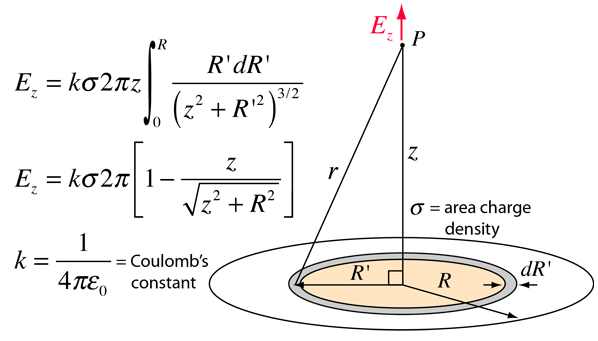
\includegraphics[width=.85\textwidth]{fig/eled.png}
	
	\caption{\href{http://hyperphysics.phy-astr.gsu.edu/hbase/electric/imgel2/eled.png}{The electrical field of a disc of charge} can be found by superposing the point charge fields of infinitesimal charge elements. This can be facilitated by summing the fields of charged rings.\label{fig:Physics-PointCharge}}
\end{figure}
\else

\fi


\ifx\magyar\undefined

\numericspanel{num:MembraneOneSegment}{The electric field of a physical charged sheet}
{
In the calculations below, we require the 'surface charge density' (interpreted as an 'infinitely thin layer' in physics, expressed in $C * m^{-2}$).
We can derive (assuming singly-charged ions) the \textit{volume charge density}
\begin{equation}
	\sigma_{V}(c) = c*N_A * e_{el} = c*6.023*10^{20} * 1.602 * 10^{-19}  = 96.5 * c\quad \biggl[\frac{C}{  mM  * m^3}\biggr]\label{eq:Physics-VolumetricChargeDensity}
\end{equation}
\noindent where $N_A$ is the number of ions in a $millimol$
and $e_{el}$ is the elementary charge. Notice that all ions contribute 
to the charge density, so simply $c=\sum_k C_k$.

Here, we run into a conflict between the 'infinitely thin'
layer of physics and the biologically implemented 
(finitely) 'thin physical layer', so we use a thickness parameter $\Delta z$.
By assuming an arbitrary 'physical layer thickness' $\Delta z$, we can calculate the  \textit{surface charge density} 
\begin{equation}
	\sigma_{A} (c,\Delta z)= 96.5*c*\Delta z \quad \biggl[\frac{C }{m^2}\frac{1}{mM * nm}\biggr] 
	\label{eq:Physics-SurfaceChargeDensity}
\end{equation}

We interpreted classical physics' notions from the theory of 'continuous' electricity,
interpreted for 'infinite' cases, for the finite world of biological objects  
and the quantized atomic world. Our idea is similar to Boltzmann's for connecting the continuous medium to particles.
When ions are present in an electrolyte having concentration $c$ 
in a 'conducting layer' of thickness $\Delta z$ on an isolating surface, they produce a field
\begin{equation}
	E_z(c,\Delta z) 
	= \frac{\sigma_A(c,\Delta z)}{\epsilon_o} =	
	10.89*10^3 * c  * \Delta z \quad 
	\biggl[ \frac{V}{m} \frac{1}{nm*mM} \biggr]
	\label{eq:Physics-ElectricFieldFromSigma}
\end{equation}
}
\else

\fi

\ifx\magyar\undefined
\subsection{Two segments\label{sec:Physics-TwoSegments}}

Now, we split the volume into two segments and compose compose the segments from 'thin physical layers' (sheets) having different concentrations (and such potentials) of ions.
We assume the membrane is transparent
for the electrical interaction (the electrical field affects the ions
in the other segment on the other side of the membrane) but not for
their masses (mechanically separates the segments). 
Separating a volume into two segments by a thin membrane has no initial effects: it actually does not affect the electrical and thermal distributions; the
\emph{bulk} concentration and potential remain the same on the two
sides of the membrane (even the double layers are electrically neutral).

We consider the immediate environment of the neuron's membrane
as adjacent parallel $(x,y)$ plates and find the electrical field's $z$ component of those plates in the points
as shown in Fig.~\ref{fig:Physics-PointCharge}. 
\hyperlink{phys:ClassicalCondenser}
{\textbf{Physics panel~\ref{phys:ClassicalCondenser}}}
discusses  the difference between the classical and biological condenser.
Furthermore,
\hyperlink{phys:CondenserBoundaryProblem}
{\textbf{Physics panel~\ref{phys:CondenserBoundaryProblem}}}
discusses 
the issues with the ill-defined biological boundaries.
\else

\fi



\ifx\magyar\undefined
We consider the immediate environment of the neuron's membrane
as adjacent parallel $(x,y)$ plates and find the electrical field's $z$ component of those plates in the points
as shown in Fig.~\ref{fig:Physics-PointCharge}.
%
In classical electricity, the charge remains on the surface of the conducting layer and the electrical field is zero inside the conducting layer; the electrical 
field contributions cancel each other.
In electrolyte segments, (a tiny fraction of) the molecules decompose into an ionized state (dissociate), see Fig.~\ref{fig:Physics-MembranePotential_Kandel6-1}, and the created ions interact with a bounding
membrane using a not entirely understood mechanism~\cite{MembraneBindingDipole:2025}.  Although not explicitly, we consider \href{https://www.sciencedirect.com/topics/engineering/electric-double-layer}{electrical double layers} to be present proximate to the membrane and ions of the dispersion medium are adsorbed on the particle's surface; depending on the chemical features of the medium.



Although it is not discussed in the classical textbooks, the rest of the dipole molecules get polarized, but do not dissociate; in this way forming virtual charges. Unlike in the conductors, the electrolyte segment next to the surface layer contains dipole molecules,
that have more or less balanced charges (the polarization depends also on the external electrical field), so they have much less mobility than the dissociated ions: their size and mass is by orders of magnitude bigger and their electrical force is a fragment of that of the ions. Their charge is virtual: it comes to light only in the appropriate environment, but creates an electrical field in the same way as real charge does. The final reason of creating virtual charges are real charges and/or external fields, so an electrical field due to virtual charges can exist also 
inside dielectrical matters such as biological cells.
\else

\fi


\ifx\magyar\undefined

%
\physicspanel{phys:ClassicalCondenser}{The classical condenser}
{
In classical electricity, the charge remains on the surface of the conducting layer, and the distribution is homogeneous (although the charge is concentrated on the surface and the electrical field is zero inside the conducting layer). Hence, the electrical field contributions cancel each other.
In electrolyte segments, (a tiny fraction of) the molecules decompose into an ionized state (dissociate), and the created ions interact with a bounding
membrane using a not entirely understood mechanism~\cite{MembraneBindingDipole:2025}. The rest of the dipole molecules become polarized but do not dissociate, forming virtual charges that allow the electrolytes to contain electrical fields. Although not explicitly stated, we assume that electrical double layers are present near the membrane, and ions from the dispersion medium are adsorbed onto the particle's surface, depending on the medium's chemical properties. 

Correspondingly, the theory non-equivocally explains the potential near the membrane surface; see the discussion and review in~\cite{SurfacePotential:1985}, mainly their Figure~1.
That model considers a symmetrical condenser, that is, both plates
contain charges of the same sign.
The Donnan function is a (discontinuous) step-like potential.
Its continuous version introduces a mathematically smooth,  non-physical function at the boundary of the charged layer.
One must describe a physically discontinuous layer (electrolyte, ion layer on the membrane's surface, and isolating membrane) with a single continuous function and gradients (potential and concentration) with physical meaning.
}
\else

\fi


\ifx\magyar\undefined
\physicspanel{phys:CondenserBoundaryProblem}
{The boundary problem of a physics condenser}
{
The behavior near the boundary layers is problematic, primarily because
the layers themselves are ill-defined.
Physically, they are not ideally plain and well-defined surfaces; the layer thicknesses are limited by the size of the ions/molecules and their associated ions; the layers do not necessarily
satisfy the ideal requirements of the respective physical laws.
Mathematically, a single 'universal' function that spans 
all regions surely cannot accurately describe the behavior
of the physical model. So, we chose a piecewise 
description where the pieces seamlessly fit at the boundaries. We assume that between the surfaces of the membrane, classical
electricity describes the electrical field; the charged layer and the electrolyte jointly produce the electrical field; we have a uniformly charged layer from separated charges on the surface and a polarized electrolyte outside them. 

Unlike in the classical theory, the electrolyte segment next to the surface layer contains dipole molecules
that have more or less balanced charges (the polarization also depends on the external electrical field), so they have much less mobility than the dissociated ions: their size and mass are bigger, and their charge is a fraction of that of the ions.  Their virtual charge becomes apparent only in the appropriate environment, yet it generates an electrical field similar to that of a real charge. The final reasons for creating virtual charges are real charges and/or external fields, so an electrical field due to virtual charges can also exist
inside dielectric matter.
We assume the membrane is transparent
for the electrical interaction (the electrical field affects the ions
in the other segment on the other side of the membrane) but not for
their masses (mechanically separate the segments). 
The membrane does not need to generate any counterforce (except for collisions).
}
\else
\fi

\ifx\magyar\undefined
\subsection{Charge layers in segments\label{sec:Physics-LayersInSegment}}

As we show, the finite thickness will result in
a lack of balance (introducing inhomogeneity and creating a voltage and concentration gradient) proximal to the surfaces of the membrane, even if the concentrations on the two sides are the same. Changing the
bulk concentration or potential in one of the segments creates a corresponding
gradient across the separating membrane, increasing the inhomogeneity proximal to the membrane.
The ions will experience an extra force due to the gradient; however, the mechanical counterforce of the membrane will keep them back in the segment. The \emph{concentration and
	potential, inseparably and having the same time course}, will change
across the two sides of the membrane, just because of the gap's physical
features the membrane represents. 

We consider that the segment is composed of electrically conducting discs (the ions are free to move on the surface), and the charged discs' contribution to the 
electrical field at point $P$ (see Fig.~ \ref{fig:Physics-PointCharge}) can be calculated as known from the 
theory of electricity. Due to the symmetry in the $z$ direction, in a homogeneous solution, the resulting electrical field in the plane perpendicular to the $z$ direction is zero, as we have contributions of equal magnitude with opposite signs.
\else
\fi

\ifx\magyar\undefined

Notice that here we used the abstraction of an infinitely thin "charged sheet", and there is a step-like
gradient in the electrical field in the gap. The physical reality is that the charge is carried by ions, which simultaneously carry mass. In equilibrium, the forces due to the voltage and concentration gradients must be counterbalanced by an external force.
%%
%Interference between scientific disciplines can also manifest here. We know simultaneously that at the boundaries of electrolytes, different interfaces, including electrically neutral electrical double layers, can be formed by only partly known 
%processes~\cite{ElectricDoubleLayer:2023}. The presence of those structures makes it hard to draw quantitative conclusions.
\else

\fi

\ifx\magyar\undefined

\subsubsection{Simple conducting sheet (a physical condenser)\label{sec:Physics-SimpleSheet}}

First, we consider a condenser that obeys 
the laws of classical electricity and has 
the geometrical size of a biological neuron.
We apply the physics terms to that pseudo-biological object
and test whether the values we derive are consistent with physiological phenomena. A tiny (according to~\cite{JohnstonWuNeurophysiology:1995}, page~12, about~$2*10^{-3}$) portion of the positive ions leaves their negative
counterions behind and forms a thin positively charged ion layer on the surface of the membrane (of course, the same happens on the opposite side with negative ions). Experience shows that -- also in biology -- two skinny layers of ions are formed on the two sides of the membrane of finite width, %\href{https://www.ncbi.nlm.nih.gov/books/NBK26910/figure/A2034/?report=objectonly}
{see the caption of figure (Fig.~11.22 in~\cite{MolecularBiology:2002})}:
"The ions that give rise to the membrane potential lie
in a thin ($< 1\ nm$) surface layer close to the membrane"
(As shown below, these ions give rise only to part of the
potential, and the dipoles in the electrolyte contribute the rest).
A sub-nanometer-thick conducting layer covers the two surfaces at the top of a $ 5~nm$-thick insulator. 
So, we model the cell with two finite-width "conductive sheet" layers.
These layers represent an electrical condenser (so we can calculate the internal electrical field between the plates) and counterbalance each other's electrical field outside the condenser.
We may assume that the solid surface provides the needed
counterforce to keep the charges at rest.

\else

\fi



\ifx\magyar\undefined
We cannot expect geometrically flat surfaces, as some biological objects of up to $1~nm$ in size are present on the surface.
So, we must assume
a physical 'uniformly charged sheet' with an average thickness $\Delta z=0.5~nm$ on the surface.
For the sake of simplicity, we assume a step-like function
for the electrical field. It is zero in the segment outside 
the "conducting sheets" (the 'bulk' portions) and inside the sheets.  Between the sheets, it jumps to the value of the electrical field of a charged sheet with surface density $\sigma_A$ (see Eq.(\ref{eq:Physics-SurfaceChargeDensity})).
(In this picture, we see a jump in the value of the electrical field
on the two sides of the physical layer. The physical layer emulates the well-defined boundary
on the side opposite to that proximal to the membrane. Here, we still assume that a mechanical counterforce due to the surface's roughness keeps the charges inside the charged layer.)

\numericspanel{num:ClassicalField}{The voltage in a classical neuronal condenser}
{
We assume that all unbalanced (dissociated) ions are in the layer,
and the rest contains no dissociated ions; furthermore, 
the ion concentration is unchanged in the segment.
In the case of a $400~mM$ solution and a $0.5~nm$ 'thin physical layer'
Eq.(\ref{eq:Physics-ElectricFieldFromSigma}) evaluates to an electrical field 
\[E^{Gap}_{Classic}(400,0.5)=0.22*10^7 \biggl[\frac{V}{m}\biggr]\]
and at a $5\ nm$ membrane thickness, the voltage across the plates becomes
%
\begin{equation}
	U^{Gap}_{Classic}(400,0.5,5)= 
	E^{Gap}_{Classic}(400,0.5)*10^{-3}* d  = 10.84\ \bigl[mV\bigr]
\end{equation}
The number of uncompensated ions needed for the cell, using the method in~\cite{JohnstonWuNeurophysiology:1995}, is $0.88*10^7$.
The calculated values are about a factor of $5$ lower than the experimentally derived values.
"An
electrical potential difference about $50-100\ mV$ ... exists across
a plasma membrane only about $5\ nm$ thick, so that the resulting
voltage gradient is about $100,000\ V/cm$"~\cite{MolecularBiology:2002}. "The number of uncompensated ions needed for the cell is $4.7*10^7$"~\cite{JohnstonWuNeurophysiology:1995}. 
}
\else

\fi

\ifx\magyar\undefined

\noindent
Based on the calculations using the classical model, the numerical figures \textbf{Numerical panel~\ref{num:ClassicalField}}
suggest our simple model to be
a strong oversimplification. 
We are in the correct order of magnitude, but we arbitrarily assumed a layer thickness, a non-dielectric medium, and a physically unreasonable step-like electrical field. 
The deviation from the expected values suggests that dipoles in the electrolyte bulk significantly alter the achievable electrical field and potential across the plates.
\begin{figure}
	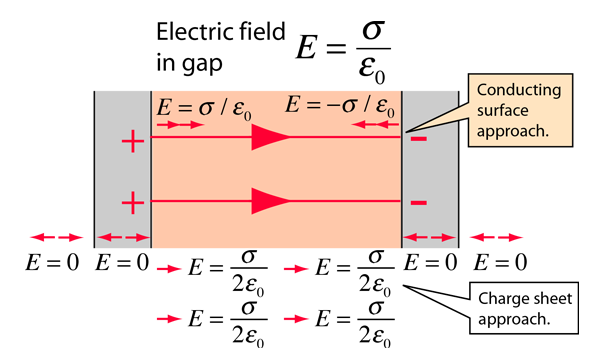
\includegraphics[width=.8\columnwidth]{fig/eplat4.png}
	
	\caption{
		The oppositely charged parallel surfaces of the membrane are treated like  conducting plates (infinite planes, neglecting fringing),
		then one can use Gauss's law to calculate the electrical field between the plates. Presuming the plates are at equilibrium with zero electrical fields inside the conductors, the result from a charged conducting surface can be used. “from Hyperphysics by Rod Nave, Georgia State University".  \label{fig:Physics-Capacitor} \copyright 
		\href{http://hyperphysics.phy-astr.gsu.edu/hbase/}{http://hyperphysics.phy-astr.gsu.edu/hbase/}
	}
\end{figure}


A usual parallel plate condenser (shown in Fig.~\ref{fig:Physics-Capacitor}) can be derived with such a model.
We have two infinite conducting sheets and 
an insulator layer between them. The magnitude of the opposite charges on the two plates must be the same as in the classical picture.
\textit{Given that the amount of surface charge densities is concluded from the ionic concentration in the segment (in a balanced state), the 
	sum of ionic concentrations of the neuron must be the same in the segments.}
A constant electrical field is present inside the membrane (across the plates of the condenser), and there is zero electrical field inside the parallel conducting plates and outside the condenser.
In this ideal picture, the charges are aligned along the boundary between two (infinitely thin) conducting layers and cannot move.
The attractive force between them and the opposite charges on the other plate 
keeps them fixed in the direction of $z$, and the repulsive force
between the charges with the same sign, the surface density in the $(x,y)$ plane remains uniform: the infinitely thin plates are equipotential.
This picture illustrates the equilibrium state of charges, consisting of infinitely small non-dissociating charge carriers and perfectly smooth surfaces. 
\else

\fi

\ifx\magyar\undefined

\subsubsection{Condenser in dielectric material\label{sec:Physics-CondenserEffect}}

In its integral form, %\href{https://en.wikipedia.org/wiki/Gauss_law}
{Gauss's flux theorem} states that the flux of the electrical field out of an arbitrary closed surface is proportional to the electrical charge enclosed by the surface, irrespective of how that charge is distributed.
The surface layer represents a steep potential and concentration gradient.
Above, we assumed that the counterforce that keeps the charges in their place
against their electrical attraction on the membrane's surface is a mechanical force: the ions cannot pass through the membrane.
However, such a counterforce does not exist on the side toward the 'bulk' part of the segment. 
The charges on the plates do not generate an electrical field
toward the bulk, but the concentration they represent does, according to the Nernst-Planck equation, provided there are charge carriers in the bulk. 
We hypothesize that virtual 
electrical charges exist in the electrolytes, and their field provides the missing electrical field.

When explaining the effect of dielectricity, we must explicitly consider the duality of ions that they obey laws of electricity and thermodynamics \textit{simultaneously}; furthermore, the complexity of the electrical structure of the solution and that the charge carriers have finite size (see "electron size" vs. "dipole size").
According to the theory of electricity, the free charge carriers (the dissociated ions) are located on the surfaces where they form powerfully charged thin layers (condenser plates) in the segments separated by a membrane on the two surfaces of the membrane; two proximal charge layers on the surfaces of the membrane.
We assume that those ions behave as point charges, i.e., 
due to the attraction from the opposite charges on the opposite plate,
they do not produce an electrical field toward
the side of the bulk of the electrolyte layers.
In the classical picture, those layers represent step-like gradients in the electrical field along the $z$ axis, and the constraint that ions must not enter the membrane provides the necessary counterforce.
\else

\fi


\ifx\magyar\undefined

From a thermodynamic point of view, a driving force acts
as long as a concentration gradient between neighboring layers exists. 
From an electrical point of view, the layers are simple parallel-plate condensers
that produce no electrical field outside their closed volume
and are connected serially; plus, the top layer has free ions. The electrical field is proportional to the bulk concentration in the layer.
Changes in the local electrical gradient may also alter the degree of dissociation and polarization, producing a graded local electrical field. 
These two driving forces have opposite directions
and in a balanced state, the same magnitude.
The counterforce acts in a way that constrains the molecules to stay in their layers; it adapts
(also compensates for the different interaction speeds)
while the gradients are changing. It presses the proximal layer against the membrane and the neighboring layers against each other.
%(In other words, the internal electrical force due to the forcefully changed polarization continuously decreases the 
%electrical field and so the potential gradient and so the concentration gradient.)


Due to the membrane's finite width and surface roughness, the conducting layer is also finite. 
The electrical field is homogeneous within the layers. The rest of that electrical field toward the bulk layer directs the dipoles proximal to the neighboring dipole layer, and their polarization increases; in other words, they "produce" an electrical field.
The final effect is that a dipole layer is attracted to
the charged layer, and it forms another layer that shows 
a charged layer toward the bulk. 
The process repeats and results in 
a decaying electrical field based on the distance from the membrane's surface.
\else

\fi


\ifx\magyar\undefined

In our model, we build the volume of the electrolyte
from thin layers of directed dipole molecules (the size of molecules limits the thinness $\Delta z$) in the volume, separated into two segments with electrolytes by a membrane with
a finite thickness~$d$ (that is, a point's distance in the electrolyte from the 
two disks will be $z$ and $z+d$, respectively). 
The contributing potential of an infinitesimal volume on the axis at point $z$ due to the charged sheet is
\[
dU(c,\Delta z,z) = 
\underbrace{E^{Gap}_{Classic}(c,\Delta z)*z}_{Potential~ from~sheet}*\frac{1}{z^2}
=  
E^{Gap}_{Classic}(c,\Delta z)\frac{1}{z}
\]
The total potential due to all elements $dz$ from the left side is (in the mathematical formulas below, we express the distance in units of $\frac{z}{d}$, so here $z$ is dimensionless).
%\begin{strip}
\begin{equation}
	U_{left}(c,\Delta z,d)=E^{Gap}_{Classic}(c,\Delta z)*d\int_{-\infty}^0\frac{1}{z} dz =\\ E^{Gap}_{Classic}(c,\Delta z)*d \biggl[\ln | z | \biggr]_{0}^{\infty}\label{eq:Physics-InternalPotentialL}
\end{equation}
%\end{strip}

In the case of a single-segment volume, within the segment, a similar potential with an opposite sign is generated by the charges on the neighboring sides of the considered charged sheet,
counterbalances the potential described by Eq.(\ref{eq:Physics-InternalPotentialL}). However, when a membrane with thickness $d$ separates the segments (with no charges in the gap), the potential on the right side will be
\begin{equation}
	U_{right}(c,\Delta z,d)
	%=E^{Gap}_{Classic}(c,\Delta z)*d\int_1^{+\infty}\frac{1}{z+1} dz 
	= E^{Gap}_{Classic}(c,\Delta z) * d *\biggl[\ln | z+1 | \biggr]_{1}^{\infty}\label{eq:Physics-InternalPotentialR}
\end{equation}
\noindent
We can write the electrical field in the form
\begin{equation}
	E(c,\Delta z,d)=
	E^{Gap}_{Classic}(c,\Delta z)*ln\biggl(\frac{z}{z+1}\biggr)
	\label{eq:ElectricFieldOutside}
\end{equation}
That is, the gap sets the potential difference across the membrane to
\begin{equation}
	U(c,\Delta z,d)=
	E^{Gap}_{Classic}(c,\Delta z) *d *\biggl(\biggl[\ln | z | \biggr]_{-\infty}^{0}-\biggl[\ln | z+1 | \biggr]_{1}^{\infty}\biggr)\label{eq:Physics-InternalPotentialFunction}
\end{equation}
We use the approximation that $\ln(\infty)\approx \ln(1+\infty)$,
and we arrive at that
\begin{equation}
	U(c,\Delta z,d)=E^{Gap}_{Classic}(c,\Delta z)*d*\biggl[ln\biggl(\frac{z}{z+1}\biggr)\biggr]_{0}^{1}\label{eq:Physics-Internal1 }
\end{equation}
\noindent describes the potential across the plates; that is,
the classical potential shall be multiplied by the result of the integral. It was experimentally confirmed~\cite{DonnanPotentialExperiental:2022} that the potential 
of the membrane is proportional to the logarithm of the distance from the membrane.
\else

\fi


\ifx\magyar\undefined

Given that the same number of charged ions must be present
on the two sides of the membrane, their resultant surface density $\sigma_A$ must be the same. 
Notice that the effect is purely electrostatic, resulting in an asymmetric ion distribution; in that balanced state, no permeability is needed. If the membrane is (slightly) permeable, ions will
move across the membrane until equilibrium is reached.
The resulting potential difference is directly proportional to the concentration difference.

The classical condenser has an electrical field, as the blue dashed line shows in Fig.~\ref{fig:The-membrane's-extra-gradient}. No field is outside the condenser or inside the condenser plates (see Fig.~\ref{fig:Physics-Capacitor}). There is a sudden jump in the field on the conductor's surface (the armatures) and a constant field between the plates.
(The charged layer can be ideally thin if electrons are sitting on the surface, but is of finite thickness on the opposite side where ions are on the surface.  This latter effect is not discussed in classical electricity.)
\else

\fi


\ifx\magyar\undefined

The biological condenser behaves differently; see the
red diagram line. An electrolyte (instead of an insulator) outside the condenser significantly alters the field's structure. The electrical field on the surface and between the plates changes by a factor of 3-4. Outside the plates, the polarization creates a field that changes logarithmically. An ion layer with finite thickness is built near the membrane's surface. It is uniformly charged, so the field inside it is linear. At the internal surface of the condenser, it takes the field value calculated for the gap; on the other side of the layer, it takes the logarithmic field value at that position. The dashed line represents the gap field, the continuous line represents the charged layer's field, and the dotted line represents the electrolyte's field. We observe the "correspondence principle": discrete and continuous fields join seamlessly; furthermore, as the electrolyte's polarizability decreases toward zero, the field approaches the classical value.
\else

\fi

%
%\subsubsection{Leakage current\label{sec:Leakagecurrent}}
%Although through $\Delta z$, the ion's water-related behavior can influence the surface charge density, one can  conclude that when only one type of ion is dissolved in the liquid, approximately the same
%concentration difference between the segments produces approximately 
%the same "thermodynamic electrical field" that can counterbalance the 
%electrical field of the biological condenser.
%
%
%
%\gls{HH} did a complete measurement, and derived \textit{precise} 
%measured data. However, their measurement was not \textit{accurate} because 
%their model was wrong.
%In a balanced state, no 
%current flows, so no voltage could be generated; see Fig.~3 in~\cite{NeuralEnergyConsumption:2017}: the leakage current is insignificant.
%More precisely: low intensity slow current flows between nearby
%ion channels inside the membrane, without involving the \gls{AIS}.
%For this reason, they assumed that a permanent leakage current $I_L$
%was flowing on the membrane, and on its resistance, it generated
%a $42.5\ mV$ voltage~\cite{CompanionGuideHodgkinHuxley:2022}.
%In \gls{HH}'s picture,
%the question \textit{what ion constitutes the current}, remains open. 
%It was claimed that the only permeability pathways open at rest are $g_{leak}$ and $g_K$. It follows that at the resting membrane potential, the leakage current equals the potassium current. That is, at rest, two currents flow (without a driving force in a balanced state), one consisting of $K^+$ ions and another of one $leakage^{+}$ ions, one generates voltage while the other not,
%and neither of them changes the concentration either on the departure or on the arrival segment, neither the concentration of the other ions; defying also Nernst's law.
%BTW: \cite{TheoryMembranePotentialEndresen:2000} discusses 
%the operation of the membrane, in some modified \gls{HH} approach: it replaces "leakage" current with "pump" currents. In the wrong model, such a modification does not matter.
%
%
%The idea of leakage current was wrong: the voltage \gls{HH} measured~\cite{CompanionGuideHodgkinHuxley:2022}  is correct, but 
%-- as our model explains -- it was generated by charge separation rather than a current through a distributed resistor.
%It is permanently present while ionic segments are on the two sides of the membrane, even when no current flows. Measuring the energy consumption of neuronal operation~\cite{EnergyNeuralCommunication:2021} confirms that no resting current,
%in the sense as \gls{HH} used the concept, exists. The existence of
%leakage current would be against, among others, the overall metabolic efficiency of 
%neuronal operation.
%The idea of leakage current, alone, undermines the credibility of the 
%\gls{HH} model as it contradicts the observed heat absorption~\cite{HeatProductionNeuron:1958} during \gls{AP}.

\ifx\magyar\undefined

\subsection{Bridging the micro- and macro views\label{sec:Physics-BridgingElectricity}}
We assumed that the function can be interpreted for regions
$(-\infty,0)$ and $(1,+\infty)$. However, we have arrived at the boundary between particles and continuous electricity.
We use a trick similar to the one Boltzmann used in his famous equation, except that we calculate the number of charge carriers from
geometrical instead of statistical assumptions.
The minimal thickness of layers is limited, at least by the size of ions.  Furthermore, the membrane's surface is not flat; there are structures (mainly proteins/lipids) with sizes of up to $1~nm$, so it is likely 
realistic to consider a layer thickness of $0.5~nm$ as we did above
(on our mathematical scale $0.1=\frac{0.5~nm}{5~nm}$), for which a multiplier of $1.7$ between the classical and the electrolytic fields exists.
A similar calculation using a layer thickness of $0.1~nm$ (on our mathematical scale, 0.02) results in a multiplier of $3.2$;
so we use a multiplier of value 3 (that corresponds to a layer thickness of $0.125~nm$ (the radius of a $Na^+$ ion is $0.116~nm$)).
Correspondingly, we assume an electrical field 
\begin{equation}
	E^{Gap}_{Dielectric}(c,\Delta z) = 3*E^{Gap}_{Classic}(c,\Delta z)  \quad 
	\biggl[ \frac{V}{m} \frac{1}{nm*mM} \biggr]
\end{equation}
\noindent
due to the dielectric properties of the segment.
This contribution arises from the dielectricity in the segment (for simplicity, we have neglected the relative permittivity). It is to be added to the value of the 
classical contribution, the 
field generated by the conducting plates, so the 
final multiplier is $4$. 
(The experience
is known in technical electricity: the \href{https://en.wikipedia.org/wiki/Electrolytic_capacitor}{electrolytic capacitors}
\textit{achieve several times higher charge storage capacity by using (\href{https://en.wikipedia.org/wiki/Pseudocapacitance}
	{pseudocapacitance})}.
Using "roughened anode foil" increases the electrolyte thickness, and the roughening provides the necessary mechanical support. 
A thicker electrolyte layer wraps the condenser plates, and the dipoles in the thicker electrolyte provide an additional charge storage facility.)
\else

\fi

\ifx\magyar\undefined
Correspondingly, 
%\begin{strip}

\begin{equation}
	E_{Gap}^{Total}(400,0.5)= 4*E^{Gap}_{Classic}(400,0.5) = 8.8*10^6 \bigl[\frac{V}{m}\bigr] \label{eq:ElectricGradient}
\end{equation}

\noindent and at a $5\ nm$ membrane thickness, the voltage across the plates becomes
%
%\begin{strip}
\begin{equation}
	U_{Gap}^{Total}(400,0.5,5)= E_{Gap}^{Total}(400,0.5) * (5*{10^{-9}}) = 45\ \bigl[mV\bigr]\label{eq:UGapTotal400}
\end{equation}
%\end{strip}
%
\noindent
"The plasma
membrane of all cells, including nerve cells, is approximately 6 to 8 nm thick and consists of a mosaic of lipids
and proteins."~\cite{PrinciplesNeuralScience:2013}, page 71.
Using such a value for the membrane's thickness may yield a thickness up to 60\% higher. 
Furthermore, the usual concentration is 
also up to 10\% higher.
Hodgkin, in 1964, measured molarity values in squid axons for ions $K^+$, $Na^+$, and $Cl^-$, (400,50,40-150) inside and (20,440,560) outside, and they provided potential values 
$55-75~mV$~\cite{JohnstonWuNeurophysiology:1995}.
Given that we used a plausible but ad hoc "charged layer thickness"
and gap distance, we cannot expect a better agreement.
However, our qualitative conclusions remain valid and can be adjusted
quantitatively to the results of dedicated measurements.
\else
\fi

\begin{figure}
	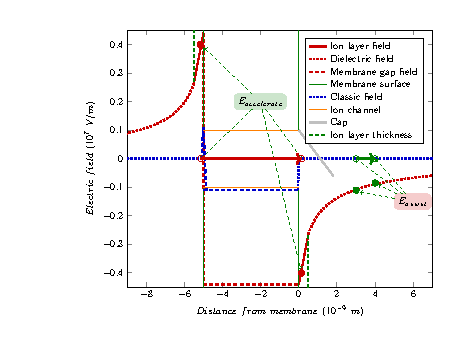
\includegraphics[width=1\textwidth]{fig/DielectricMembrane.pdf}
	\caption{The neuronal membrane's \emph{electrical field} in the function
		of the distance from the membrane's surface.
		The thickness of the 'atomic layers' proximal to the membrane's surfaces
		are also shown.
		The electrical field is linear inside the uniformly charged atomic ion layer on the surface and is described by Eq.(\ref{eq:ElectricFieldOutside}) in the electrolyte.
		For visibility, a layer thickness $0.5\ nm$ is assumed.
		For illustration, a simple capped ion channel in the membrane's wall
		is also displayed. \label{fig:The-membrane's-extra-gradient}}
\end{figure}


\ifx\magyar\undefined
We have the boundary conditions that we know the electrical field at the membrane's surface through the volume charge density, and the Nernst-Planck equation delivers the change
of the electrical field due to the change in concentration. 
The physical constraint is that the layer thickness
cannot be infinitely small. If we use a parameter for layer thickness equal to that of the surface layer, 
the calculated electrical field distribution will be
scalable. 
\else
\fi

%\subsection{The dynamic layers\label{sec:Physics-DynamicLayer}}
%This layer's importance and operation are in
%line with the Earth's atmosphere. Its features drastically deviate
%from the features of the bulks on its two sides. It is separated by
%a sharp contour on one side and an ill-defined border on the other;
%its volume is far from being homogeneous. Gravity keeps it in place, and it is at rest. However, sometimes,
%for some periods, also other (thermodynamic and electrical) forces are evoked
%inside it and lead to transient changes, moving huge masses with high speeds
%inside it. Their thickness and mass are negligible compared to those
%of the bulks on their two sides, and we can describe the bulks without
%considering their density, mass, size, etc. Still, this thin layer is
%responsible for the weather.
%%; its transient processes define the visibility
%%from both sides (define propagation of electromagnetic fields), and
%%it can protect us from 
%%\gls{EM}
%%EM radiations.
%It can temporarily absorb
%products of slow processes (water evaporation) and deliver masses of
%high density (much above its density, such as water, sand, etc.) to
%continental distances, creating the illusion that it temporarily stores that matter.
%Minor changes (natural ones, such as a slight difference in air temperature, and artificial ones, such as injecting condensation nuclei in clouds)
%can result in enormous changes. We can even imagine volcanic eruptions
%as semipermeable gates for material with apparently random operation
%and distribution of the injected material.
%
%To describe those complex and continuous phenomena at least approximately,
%we must separate them into stages. We can describe the stages approximately using omissions, approximations, and
%abstractions, usually considering
%only one dominant phenomenon. The described phenomena are interrelated
%in a very complex way and depend on different parameters. To some
%point, we can describe that thin layer using a static picture and
%provide an empirical description of its processes, even though 
%we can give some limited validity mathematical descriptions for those
%stages. However, we understand that for describing the time course of the transition
%(contrasting with step-like stage changes) between those well-defined
%stages of the atmosphere, we need a \emph{dynamic description} to
%discover the \emph{laws of motion} governing the processes.
%
%The same is true of neuronal membranes and neuronal function.
%Now, we are at the point where their decades-old static description
%is insufficient. We need
%to derive the corresponding laws of motion to describe the neuron's dynamic behavior. We need a meticulous and
%unusual analysis to derive them. 
%%
%In a neuron, in the abstraction science uses, we put together only
%an ionic solution, a semipermeable membrane, and currents that enter and leave
%it. All these belong to non-living matter.
%As experienced, \textit{at some combination of their parameters and gradients, qualitatively
%	different phenomena happen, which, in the abstraction biology uses,
%	are called signs of life};
%our system starts to belong to living matter.
%Given that the approximations, the derived abstractions,
%and the mathematical formalisms describing them are different for
%the two cases, \emph{it looks like we have two different, only loosely
%	bound worlds}. We realize we have arrived at the boundary of non-living
%and living matters, and we must go back to the \emph{first principles
%	of science} to clarify where their boundary is. However, by using our approach, we may defy that "the
%emergence of life cannot be predicted by the laws of physics"~\cite{ConservationOfInformation:2021}.
%Our artificial duck looks, quacks, and swims like a duck. 



\ifx\magyar\undefined

\section{Forming membrane's potential\label{sec:Physics-FormingPotential}}

In this section, we model the neuron as an electrical circuit that comprises an electrolyte condenser implemented by its membranes, surrounded by two electrolyte segments. The membrane comprises low-transmission-capacity ion channels in its wall and high-transmission-capacity channels toward its axon; it also uses slow ions rather than electrons.
The condenser produces a potential (that depends on the membrane's thickness and the concentrations in the two segments, as discussed above).  Furthermore, the two electrolyte segments produce Nernst voltages that are combined to yield a single voltage. 
According to Kirchhoff's Voltage Law, in a balanced state, the sum of those voltages between the intracellular and extracellular segments must be zero.
However, one must take into account the effects of the "slow current" (emulated by 
"fast current" with a plausible time course in the simulator).
We omit biological regenerative processes (such as \gls{ATP} production via hydrolysis, ion pumps and channels functioning, and so on) and discuss only the most important physical primary processes.
In light of our findings, we must reconsider several key concepts in neurophysiology.


The electrical processes are inseparable from the corresponding thermodynamic processes~\cite{VeghNonOrdinaryLawsForLife:2025}, which we discuss by deriving an "equivalent thermodynamic electrical field" in section~\ref{sec:Physics-ElectrolyteInhomogeneity}.
The other minor effect is a low-intensity "passive flux" produced by the
"resting channels". They are different from the ion channels in the \gls{AIS}~\cite{AIS_NeuronalPolarity:2010, ActionPotentialGenerationNatrium:2008, BackpropagationAP:2012, AIS_Updated_Viewpoint:2018, AISStructureReview:2018}.
The "resting current" is about two orders of magnitude lower~\cite{EnergyNeuralCommunication:2021,NeuralEnergyConsumption:2017} than \gls{HH} assumed at the time of writing their papers; correspondingly, its role is much smaller in the transient state, and it even drastically changes the electrical model used in producing an \gls{AP} which we discuss elsewhere~\cite{VeghDANCES:2026}.
\else

\fi


\ifx\magyar\undefined
\subsection{States\label{sec:PHYSICS_STATES}}

Figure~\ref{fig:NernstPlanckThermalWidth} shows, in the function of the membrane's thickness, the electrical field across the membrane due to electrical charges (it does not depend on the thickness of the membrane), for different physically plausible assumptions; furthermore, the thermal electrical field. The two electrical fields show significantly different dependencies on the neuron's parameters. Recall that although the parameters we used are biologically plausible, they are only estimations from non-dedicated, incomplete measurements. The qualitative conclusions, however, remain valid. 

The balanced state is set where the thermodynamic and electrical "electrical field" diagram lines cross each other; 
around $5\ nm$; the value we assumed in evaluating our equations.  
On the other hand, we can check the electrical field's dependence on the summed-up concentration of the ions in the segment (see Fig.~\ref{fig:NernstPlanckThermalConcentration})
(dehydration, for example, changes the setpoint through changing concentrations).
Here, the thermodynamic electrical field is constant but different at different width parameters. The field of the classical condenser does not provide a reasonably balanced state (a matching line). The dielectric diagram line seems to provide a realistic estimation 
when using biologically reasonable parameters. 
One can describe the neuron as a balanced system at the intersection of the sloping and the horizontal lines. In the resting state, only minor deviations (fluctuations) from this state exist
in both the electrical field and the chemical concentration. 
\else

\fi


\ifx\magyar\undefined

\begin{figure}
	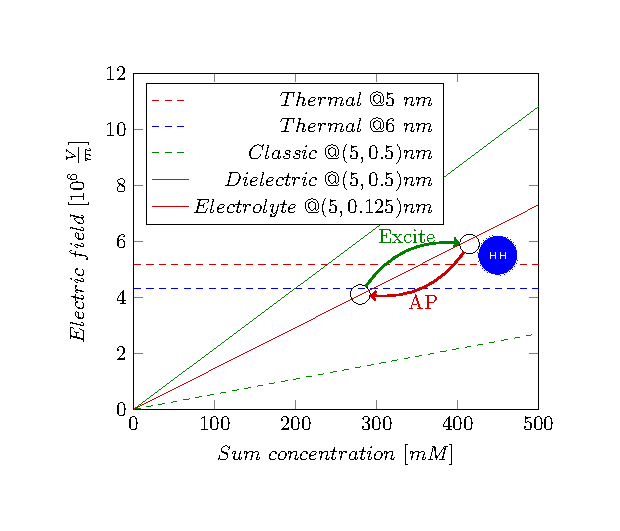
\includegraphics[width=.8\columnwidth]{fig/NernstPlanckConcentration.pdf}
	\caption{The electrical and the thermal "electrical fields" at different concentrations, see Eq.(\ref{eq:ElectricGradient}). The thermal electrical field varies with the thickness parameter and depends on the concentration; see Eq.(\ref{eq:NernstPlanckThermal2}). Balanced states are where 
		the sloping lines cross the horizontal ones. The dot marks where \gls{HH} provided measured data.
		\label{fig:NernstPlanckThermalConcentration}
	}
\end{figure}


In the transient state, if we assume that a charge transfer causes a significant potential change around $100\ mV$ in the layer of width 
$10\ nm$, it means a $10^7 \bigl[\frac{V}{m}\bigr]$ jump in the electrical field that is caused by a $100 \bigl[mM\bigr]$ jump in the concentration (for only a short time and only in the mentioned layer, but not in the bulk; see also Fig.~\ref{fig:RestingPotential4}). One can infer that a neuron can minimize its offset voltage (and so: its energy) by either decreasing its membrane's width, the sum concentration of the electrolyte, the electrical field, or by a process with a temporal course that changes their combination, thereby implementing a true multi-physics phenomenon. During issuing an \gls{AP}, the system finds its way back to the crossing point (the path in the phase space is not simple: concentrations on both sides of the membrane and the electrical field in the mentioned layers change, all having different speeds; electrical, thermodynamic, mechanical and so on, changes happen; the process is a relaxation (a waving), as it is seen in the shape of an \gls{AP}). 
\else

\fi


\ifx\magyar\undefined

We can imagine how the electrical process occurs in this 
controlled system (for visibility, the positions of the marks are not proportional to the mentioned numbers). The system is in a balanced state at a crossing point. The two circles connected by bent arrows represent that when an excitation begins at the point with lower
concentration and higher potential (the cytoplasm side and negative resting potential), ions rush into the surface layer, so the ion concentration increases, which increases the electric
field; this is seen that the membrane potential suddenly increases. (We note here that, due to ions' repulsion, the pressure also increases proportionally with the potential.)
The increased potential starts a current, but the current is slow,
and the intensity of the current through the channels in the
membrane's wall is much lower than the current of the drain (\gls{AIS})
so the system issues an \gls{AP} as it returns to its (balanced) starting point.
Given that it receives a large amount of $Na^+$ ions,
its primary effort is directed to get rid of them (the electrical gradient 
cannot distinguish the electrical charges by their chemical nature),
so the output current through the \gls{AIS} comprises mainly
$Na^+$ ions.
The system will move along a line, with the restriction that it is a movement in phase space (the change in concentration is not proportional to time), and the different points on the membrane's surface may have different potentials at different times (spatiotemporal behavior). Due to the capacitive current, the local potential may temporarily drop below the setpoint (as observed in physiology, this phenomenon is known as hyperpolarization). The time course of the processes is described by the laws of motion of biology~\cite{VeghNonOrdinaryLawsForLife:2025} (the time derivatives of the Nernst-Planck equation). The simplified model operates as described in section 4 of~\cite{VeghTechnomorphBiology:2025} and its computational details are provided  in~\cite{VeghNeuronAlgorithms:2025}.

\textit{Based on the correct physical model, we can get closer to understanding and reducing the effects of neurological diseases~\cite{AlzheimerDisease:2022,ParkinsonDisease:2024},
which is not possible while having a wrong model in mind,
with batteries and autonomously changing resistors inside the neuron.} 
The change in parameter values potentially leads to neurological diseases as suspected: "Structural alterations of the \gls{AIS} are likely to have an impact on normal neuronal activity”~\cite{AlzheimerDisease:2022}. 
When lipid debris accumulates on the surface of the neuron membrane~\cite{AlzheimerDisease:2022}, the thickening of the layer $\Delta z$ reduces the electric field strength (i.e., changes the neuron's 'setpoint'). In that case, the resting potential (and the threshold potential) may change, which weakens \gls{AP} generation.
The elongated shape of the neuron means that the resistance of the 
\gls{AIS} increases that changes the parameters of the \gls{AP};
see Eq.(\ref{eq:AIS_Voltage}).
"In brain tissue from Alzheimer’s disease patients \dots the most common changes were a proximal shift or a lengthening of the AIS"~\cite{AlzheimerDisease:2022}.  
Also, as~\cite{TemperatureOnAP:2022} observed, the setpoint changes with temperature (the "thermodynamic electrical field" changes with the temperature, while the "electrical electrical field" does not, so their crossing point changes), reflected in the dynamics of the \gls{AP}.
\else

\fi


\ifx\magyar\undefined

\subsubsection{Resting state\label{sec:PHYSICS_RESTINGSTATE}}
In the resting state, the goal is to provide stability with slow, less intense currents. As~\cite{PrinciplesNeuralScience:2013} discusses, there are 'holes' (non-controlled ion channels) in the membrane where the counterforce is missing, so
the difference in the electrical and thermodynamic forces could accelerate ions until the Stokes-Einstein speed (see Eq.(\ref{eq:StokesEinsteinSpeeddV})) is reached.
Given that the deviation from the setpoint is slight, the current's intensity and speed are low. 
The slow ion transport delivers both charge and mass, so the gradients
permanently direct the process control variable toward the reference point. Given that the 'resting channels' are scattered on the surface of the membrane and it takes time for the gradients delivered by slow ions to reach the entrance of an ion channel, some slight variations 
in the actual value of the membrane's potential necessarily exist.
Given that the \gls{AIS} comprises non-gated ion channels with much higher density than those in the membrane, the variations and the control ("leaking") are marginal, and the current flows mainly through the ion channels in the membrane's walls, as observed in experimental physiology.
\else

\fi


\begin{figure}
	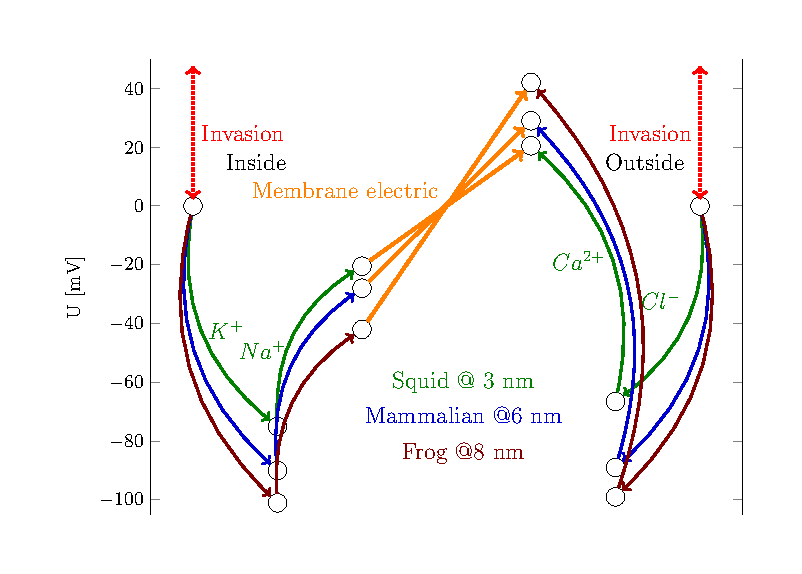
\includegraphics[width=.8\columnwidth]{fig/RestingPotential3.pdf}
	\caption{The mechanism for controlling neuronal operation is the same in all cases shown in Table~\ref{Tab:SummaryTable}. It appears that 
		the thicker membrane produces a higher membrane electrical potential, requiring a higher thermal potential to compensate. However, it can solve the task using a lower salt concentration, since the electrical membrane potential accelerates ion flow through the membrane channels, thereby speeding up the operation. The electrical fields for the different species have similar values, as shown in  Fig.~\ref{fig:NernstPlanckThermalWidth}.
		Furthermore, 
		the total concentration decreases as the membrane thickness and potential increase.  
		\label{fig:RestingPotential3}
	}
\end{figure}


\ifx\magyar\undefined

In Fig.~\ref{fig:RestingPotential3}, the electrical voltage contribution is unidirectional. In contrast, the two-component thermodynamic contributions, which depend on the concentrations, are bidirectional.
If choosing the zero potential at the middle of the electrical potential, we can interpret that
the concentration combinations maintain their ionic concentrations (and so also thermodynamic voltage contributions) independently on both sides, starting from a zero potential level. They generate potentials autonomously in the segments proximal to the opposite membrane surfaces. The electrical charge on the membrane generates an additional voltage independently. However, that voltage must fit between the two thermodynamic voltages. Any deviation in potential between the intracellular and extracellular sides initiates a current that drives the concentrations and voltages toward a balanced state.
The process is complex: the sum of surface concentration of ions must be the same on both sides for the condenser, and the ratios on the intracellular and extracellular sides must be adjusted to satisfy the conditions 
%% LaTeXML error
%\begin{align}
%	U_{internal}^{K^+,Na^+} &= -U_{electric} &+ U_{internal}^{K^+} &+ U_{internal}^{Na^+}&(+U_{internal}^{invasion})\\
%	U_{external}^{Cl^-,Ca^{2+}} &= U_{electric} &- U_{external}^{Cl^-} &- U_{external}^{Ca^{2+}}&(+U_{external}^{invasion})
%\end{align}

In a balanced state, the left sides are zero: at the contact point between the electrolyte and the membrane,
there are no potential differences, while in a perturbed state, they are non-zero and so they represent driving forces for restoring the balance. (Recall that the ions are slow and that the local electrical and concentration gradients control the local potentials.)
From the derivation, it follows that
%\begin{align}
%	U_{electric} &= - 2*(U_{internal}^{K^+} &+ U_{internal}^{Na^+}) \\
%	U_{electric} &= - 2*(U_{external}^{Cl^-} &+ U_{external}^{Ca^{2+}}) \\
%	U_{electric} &=  U_{internal}^{K^+} &+ U_{internal}^{Na^+} 
%	&= - (U_{external}^{Cl^-} &+ U_{external}^{Ca^{2+}})\quad
%\end{align}
\else

\fi



\ifx\magyar\undefined
Our statement is the precise mathematical formulation of that
"Thus ions are subject to two forces
driving them across the membrane: (1) a \textit{chemical
	driving force}, a function of the concentration gradient
across the membrane, and (2) an \textit{electrical driving force},
a function of the electrical potential difference across
the membrane."~\cite{PrinciplesNeuralScience:2013}, page~129.
%and that "nerve and muscle cells
%have a particularly rich variety and high density of
%membrane ion channels; their channels do not differ
%fundamentally", page~107
Fig.~\ref{fig:RestingPotential3} quantitatively underpins that "action potential generation in nearly all types of neurons and muscle cells is accomplished through mechanisms similar to those first detailed in the squid giant axon in early research by \gls{HH}"~\cite{MembranePotentialMoleculesNetworks:2014}. \textit{In all species, the chemical and thermodynamic processes keep a balance in the cells of different construction in both resting
	and transient states.}

According to the above derivation, we consider three characteristic segments in the neuron. In the middle, we have an electrostatically charged isolator plate with positive and negative charge carriers on its two surfaces and none inside, so it has a homogeneous electrical field. The magnitude of the field depends only on the total concentration of the corresponding ions in the segments. On both sides are ionic solutions of different compositions. If the membrane is permeable for the ions, they can move from one segment to the other as the resultant field dictates,
until the fields get balanced.
\else

\fi



\ifx\magyar\undefined
The membrane's electrical potential defines the resting potential, and the "electrical" and "thermodynamic" potentials work together to control neuronal operation.  
The anatomically defined "electrical" membrane potential, combined with the vast number of ions in the extracellular space, provides a stable concentration that serves as a solid reference point (a setpoint).
In the resting state, the membrane potential is balanced by the presence of always-open "resting ion  channels". When ions flow
into the membrane, the "resting ion  channels"
can keep the balance: the internal $K^+$ and $Na^+$ concentrations are adjusted as the $Na^+$ flows in.

Figure~\ref{fig:RestingPotential3} also shows that
in its native state, the neuron is electrically balanced: in the
internal and external segments, the resulting thermodynamic and electrical forces are equal.
Any foreign invasion into the neuron's life (chemical, mechanical, or electrical, including clamping) changes the left-side reference value to
an externally set value. The neuron must adjust its $Na^+$ and $K^+$ concentrations to reach a new balance while the invasion persists. That is, any invasion ("testing in the physical laboratory") changes the concentrations and voltages 
inside the cell. In addition, the internal biological processes can trigger internal processes that contribute (from the measurement's point of view) foreign currents or processes, see also section~\ref{sec:TransientState}. The feedback from the clamping methods introduces a compensating current. Even a simple conductance-measuring device is active: it applies a test voltage that generates a test current, which can sensitively affect the ionic composition of the neuron (recall that concentrations may differ by up to six orders of magnitude). Although modern electronic devices attempt to conceal this effect, they subtly influence biological operation.
\else

\fi

\ifx\magyar\undefined
From our result, it follows that for more chemical elements, a per-element coupled set of equations exists, plus the sum concentration
agreed electrical fields that are valid simultaneously and define the process variable (aka membrane potential) of the neural regulatory circuit.
In a more symmetrical form

\begin{align}
	0 &=\frac{U_{electric}^{Total}(c,\Delta z,d)}{2} + \sum_k U_{thermal}^{C_k}(d) + {invasion}
	\quad for\ all\ k;\ inside\ and\ outside \\
	c &=\sum_k C_k^{ext} =\sum_k C_k^{int}	\label{eq:coupling}
\end{align}
In the classical measurement by \gls{HH}, the sum of the concentrations of $K^+$ and $Na^+$ in the cytoplasm and extracellular fluid  (in mM) is 380 and 390, respectively, while the  concentration of the $Cl^-$ %(and $Ca^{2+}$)
are 450 and 460; practically all equal, as our analysis has derived.  The deviations are well within the uncertainty of the 
measured values. 
\else

\fi
 

\ifx\magyar\undefined
That is, we have an unidirectional electrical potential difference and oppositely directed thermal voltages. In the balanced state, the two potentials must be equal.
When changing, say, one concentration, the other concentration on the same side, and the surface charge density of the condenser, changes accordingly.  The changed electrical voltage 
re-adjusts the thermodynamic voltage and, consequently, the concentrations in the other segment.
There is no simple way to express, say,
$[Na^+]_i$ in the function of $[K^+]_i$ or vice versa, and similarly for the other ions. Everything moves.
The size matters: the amount of ions in the external segment is many orders of magnitude higher, and the gradients are inversely proportional to that amount.

As the figure suggests, an external invasion, typically an electrical voltage on the intracellular side, changes the balanced state, and due to the parameters being linked,
changes all concentrations. When moving the system out of
its balanced state, in any way, a driving force appears that moves the system towards finding a new balanced state. However, recall that the ions are slow, so \textit{the changes are not instant}.
\else

\fi
%
%Table~\ref{Tab:SummaryTable} shows our results for three different
%famous published cases (Table 2.1 in\cite{JohnstonWuNeurophysiology:1995}). It looks like the calibration of the concentration 
%of negative and positive ions needs scaling, and the measurement of $Ca^{2+}$
%comprises issues (the $Ca^{2+}$ concentration in all cases is inaccurate and had to be corrected).
%
%\renewcommand{\arraystretch}{1.3}
%\begin{table}
%	\caption{The summary data table for equilibrium (Data from Table 2.1 in\cite{JohnstonWuNeurophysiology:1995} ) \label{Tab:SummaryTable}}
%	\begin{tabular}{ |p{0.6cm}||p{0.7cm}|p{0.9cm}|p{3.0cm}| p{0.85cm}| p{0.85cm}| p{0.95cm}|p{0.65cm}|p{0.90cm}|}
%		\hline
%		\hline
%		Ion& Inside &Outside &  $U_{therm}\frac{RT}{zF} log\bigl( \frac{[C]_{o}}{[C]_{i}}\bigr)$ &$U_{electr}^{theor}$&$U_{electr}^{exper}$&$U_{membr}$&Width&$E_{membr}$\\
%		& [mM] & [mM] &  [mV] &  [mV] &[mV]&[mV]&[nm]&[MV/m]\\
%		\hline
%		&\multicolumn{6}{|c|}{Squid (\gls{HH}) \quad T=293\ $K^o$}&\textbf{3}&14.0\\
%		\hline
%		\em	$K^+$ & 400 & 20 & $-75.5= 58 log\bigl( \frac{20}{400}\bigr)$& \textbf{41.9}&\textbf{41.4}&-62.0&&\\
%		$Na^+$ & 50 & 440 & $+54.8= 58 log\bigl( \frac{440}{50}\bigr)$&&&&&\\
%		$Cl^-$ & 40 & 560 & $-66.5= 58 log\bigl( \frac{560}{40}\bigr)$&\textbf{41.9}&\textbf{42.0}&63.0&&\\
%		$Ca^{2+}$ & $0.27^*$ & 10 & $+45.5= 29 log\bigl( \frac{10}{0.27}\bigr)$&&&&&\\
%		&\multicolumn{8}{|l|}{$^*$ used for the published value 0.4} \\
%		
%		\hline
%		&\multicolumn{6}{|c|}{Frog muscle (Conway) \quad T=293\ $K^o$}&\textbf{8}&9.61 \\
%		\hline
%		$K^+$ & 124 & 2.25 & $-101= 58 log\bigl( \frac{2.25}{124}\bigr)$&\textbf{88.9}&\textbf{83.6}&-125.4&&\\
%		$Na^+$ & 10.4 & 109 & $+59.2= 58 log\bigl( \frac{109}{10.4}\bigr)$&&&&&\\
%		$Cl^-$ & 1.5 & 77.5 & $-99.4= -58 log\bigl( \frac{77.5}{1.5}\bigr)$&\textbf{88.9}&\textbf{82.7}&124.1&&\\
%		$Ca^{2+}$ & $0.021^*$ & 2.1 & $+58.0= 29 log\bigl( \frac{2.5}{0.25}\bigr)$&&&&&\\
%		&\multicolumn{8}{|l|}{$^*$ used for the published value 4.9} \\
%		
%		\hline
%		&\multicolumn{6}{|c|}{Typical mammalian cell \quad T=310\ $K^o$}&\textbf{6}&11.1 \\
%		\hline
%		$K^+$ & 140 & 5 & $-89.7= 62 log\bigl( \frac{5}{140}\bigr)$&\textbf{57.7}&\textbf{57.3}&-85.8&&\\
%		$Na^+$ & 15 & 145 & $+61.1= 62 log\bigl( \frac{145}{15}\bigr)$&&&&&\\
%		$Cl^-$ & 4 & 110 & $-89.2= -62 log\bigl( \frac{110}{4}\bigr)$&\textbf{57.7}&\textbf{56.9}&85.9&&\\
%		$Ca^{2+}$ & $0.04^*$ & 5 & $+60.8= 31 log\bigl( \frac{5}{0.04}\bigr)$&&&&&\\
%		&\multicolumn{8}{|l|}{$^*$ used for the published value 0.0001} \\
%		
%		\hline
%		&\multicolumn{6}{|c|}{$Na^+$ ions only~\cite{OriginMembranePotential:2017}\quad T=310\ $K^o$}&6&10.0 \\
%		\hline
%		$Na^+$ & 12 &145 &$+66.6= 62 log\bigl( \frac{145}{12}\bigr)$&\textbf{60.7}&\textbf{66.6}&&&\\
%		\hline
%		\hline
%	\end{tabular}
%\end{table}
%
%When calculating the values in Table~\ref{Tab:SummaryTable}, we used $\Delta z=1.05$ and employed the membrane thickness data from various publications to demonstrate that our theoretical approach is correct and that using the correct data can yield even the absolute values of the membrane potential.   
%The higher-than-expected value of $\Delta z$ may suggest that the ions and the membrane's double layers in the electrolyte may also play a role. 
%Dedicated, complete investigations can reveal the details.
%
%
\ifx\magyar\undefined

\subsubsection{Transient state\label{sec:TransientState}}


\begin{figure}
	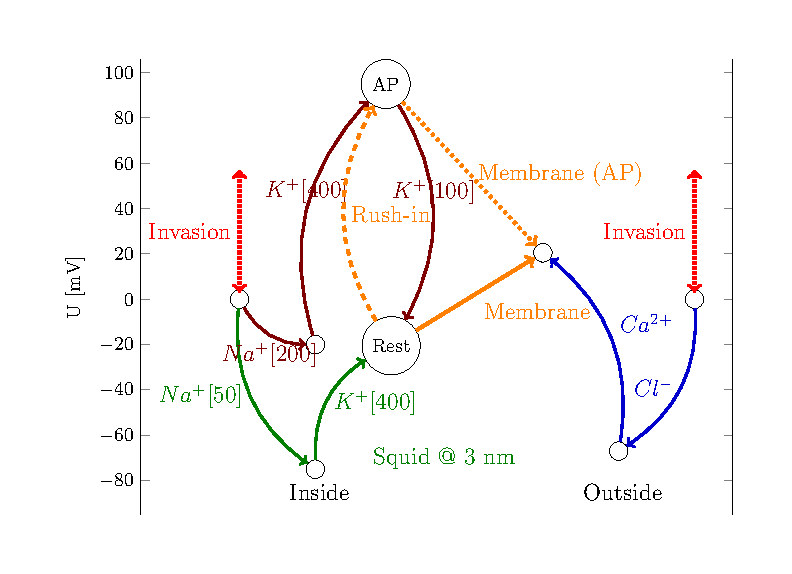
\includegraphics[width=.8\columnwidth]{fig/RestingPotential4.pdf}
	\caption{The mechanism of producing \gls{AP} (using numbers referring to the case of squid shown in Table~\ref{Tab:SummaryTable}). In the resting state, the inside thermal potentials follow the green paths.
		When the rush-in of $Na^+$ ions suddenly increases the internal concentration to $[200]$, the potential on the internal side of the membrane increases to $+90\ mV$. The neuron must decrease its $Na^+$  concentrations to restore the resting potential, mainly by releasing an action potential through the \gls{AIS}.
If the clamping fixed the mebrane's voltage at the peak voltage of the \gls{AP}, the neuron must release $K^+$ ions until its reaches concentration [Na50,K7].	
		\label{fig:RestingPotential4}
	}
\end{figure}

In a special type of invasion, when suddenly a large amount of $Na^+$ rushes in (i.e., the trigger is external, but the ions derive from a biological process),
the current throughput of the "resting ion channels" 
is not sufficient anymore: the internal $Na^+$ concentration in the proximal layer drastically increases, and so does the 
membrane's potential. At that point, the neuron is out of balance: although most of the $Na^+$ ions can
flow out through the \gls{AIS}, the system also changes its $K^+$ concentration through the limited capacity "resting ion channels" until the balanced state is regained. This latter effect must not be confused with the capacitive current, which (owing to its reversed direction) causes the phenomenon known as "hyperpolarization".
\else

\fi


\ifx\magyar\undefined

Compare the figure to Fig.~7.2 in~\cite{PrinciplesNeuralScience:2013}.
Notice the two-sided negative feedback effect: a change in the value of the 
"command potential" or "command concentration" (the "setpoint" in the language of control theory) changes the other value.
In the case of voltage invasion, the ion concentration ratio also changes. In this case, the feedback amplifier is represented by the 
delicate balance of the electrical and thermodynamic force fields.
In the case of clamping, another (electrical) feedback amplifier is introduced
into the system, and they work against each other. The neuron attempts 
to restore its balance without external potential (it cannot distinguish the foreign potential from its membrane potential), and changes its concentrations accordingly.
A vital difference is the \textit{speed} of the feedback amplifier. The electrical one operates at electrical speed (not considering the electrolyte electrodes), while the thermodynamic one operates at a speed several orders of magnitude lower.
When switching (or changing) the external ("command") voltage,
the neuron must first get into its "steady state". It takes time.
"The command potential, which is selected
by the experimenter and can be of any desired amplitude
and waveform"~\cite{PrinciplesNeuralScience:2013}. However, if the measured data readings are not from a steady state,
the measurement is wrong: the different amplifier speeds (different current speeds) surely distort the measured value. 



Figure~\ref{fig:RestingPotential4} shows the schematic course of potentials and concentrations during issuing an \gls{AP}. 
Follow the green path: the concentration ratio of 
$Na^+$ and $K^+$ ions define a thermodynamic contribution in the intracellular segment. Follow the 
blue path: the $Cl^-$ and $Ca^{2+}$ ions define a thermodynamic contribution in the extracellular segment.
%
On the left side, two positive ions are in the solution, and the membrane potential (due to charge separation) rises toward the outside segment; the ions cannot go "uphill". Similarly, 
the $Cl^-$ ions cannot go uphill (due to their negative charge, the same potential is also rising for them). This single membrane potential keeps all ions in their segments. However, the $Ca^{2+}$ ions can travel "downhill".
Calcium pumps are needed: although in minimal concentration, $Ca^{2+}$ ions flow into 
the intracellular segment, and they must be pumped out (BTW: this is likely also the reason why measuring $Ca^{2+}$ concentration is inaccurate).
\else

\fi



\ifx\magyar\undefined
As discussed above, 
the concentrations and voltages in the extracellular segment, with their vast amount of ions, remain unchanged
in resting and transient states.
Follow the red path: $Na^+$ ions rush into the intracellular segment.
They increase the concentration from $[50\ mM]$ to (say) $[200\ mM]$
(from point (Rest) to point (AP)). This sudden change increases the thermal contribution of $Na^+$ potential to $[-20\ mV]$, but 
because the total charge on the membrane significantly increases, the resulting voltage on the intracellular side of the membrane increases to $[90\ mV]$.
The neuron could decrease its potential to the resting value if it could decrease the $K^+$ concentration to $[100\ mM]$. However, the ion-delivery capacity of the "resting ion channels" is insufficient: they are sized to maintain the resting state.
(Furthermore, the electrical contribution appears instantly, while the thermodynamic one, due to the finite speed of ions, only with some delay~\cite{VeghNonOrdinaryLawsForLife:2025}.)
Follow the dashed orange path: the large amount of rush-in $Na^+$ ions drastically increases the surface concentration on the membrane, so the potential suddenly changes to $[90\ mV]$. Follow the dotted orange path: the electrical field across the membrane suddenly changes its direction from positive to negative (see the slopes of the solid and dotted orange lines) so that the excess positive ions can move "downhill" out of the intracellular space through the high-conductance ion channel array (\gls{AIS}) at the end of the neuron.
Its internal end is at the high membrane potential,
while the external end is at the low potential of the extracellular segment. 


The setpoint on the extracellular side remains fixed.
On the intracellular side, at the beginning of the \gls{AP}, the actual voltage 
is above that of the setpoint on the extracellular side, so at the two ends of the \gls{AIS}, a positive driving force moves the ions toward the downstream neuron. 
Given that positive $Na^+$ ions leave the intracellular segment, its potential continuously decreases. At some point, 
\textit{the voltage drops below the setpoint of the extracellular side,
	and the electrical field across the membrane reverses}. 
The driving force also decreases, and a low-intensity current
restores the balanced state to the previous setpoint.
When measuring at the \gls{AIS}, one observes that the
potential rises suddenly, then decreases below the setpoint (hyperpolarizes the membrane), then a decreasing current (flowing in the opposite direction due to the changed slope of the resulting potential, the changed electrical field across the membrane,
but comprising the originally rushed-in $Na^+$ ions) slowly restores the resting potential.
Here comes the finite speed of ions again. 
The ions can follow the potential changes with a delay
due to their finite speed, causing an apparent delay in the time course of the \gls{AP}'s current. 
\else

\fi

\ifx\magyar\undefined
Models in neuroscience (as reviewed in~\cite{BrainNetworkModels:2018})
almost entirely ignore these aspects. In our physical model, we see
that the measurable membrane potential and current change in the function
of the ions' speed, the concentration, and its time derivative.
Furthermore, all mentioned quantities depend on the effective potential. 
As Eq.~(\ref{eq:NernstPlanckThermal1}) shows, the "thermodynamic electrical field" increases
as the temperature increases, and raises the setpoint.  As Eq.(\ref{eq:StokesEinsteinSpeeddV})
shows that the current decreases as the temperature increases, in line with the experimental evidence~\cite{APTemperatureDependence:2012,APTemperatureDependence:1985}.
The amplitude of the action potential is decreased, given that the setpoint has increased, and its duration is reduced, given that the current decreases.

\else

\fi


\subsection[Controlling states]{Controlling neuronal stages\label{Physics-ControlTheory}}

From control theory, it is known that the goal of a controlled system is to
govern the application of system inputs to drive the system to a desired state while minimizing delay and overshoot, steady-state error, and ensuring control stability.
The neuron implements a controller that monitors the controlled process variable (membrane voltage) and compares it with the reference or setpoint (resting potential).
Recall that the geometry and the composition and concentration of electrolytes define the setpoint. 
The difference between the process variable's actual and desired values, known as the error signal, represents the actual offset potential.
It is applied as feedback to generate a control action that brings the controlled process variable to its setpoint.

\subsubsection{Neuron as a PID controller\label{Physics-PIDController}}

Biology uses a simple \gls{PID} controller with proportional, integral, and derivative components. 
In simple words, it means that the output of the system (the output voltage measurable on the \gls{AIS}) depends on the input voltage (the present: input current if the resistance is constant),
the integrated input current(s) (the past), and their derivatives (the future). Notice that calculating the derivatives of the interdependent parameters needs care, as discussed in~\cite{MechanicalPropertiesNerves:2025}. The sum of those summands defines the resulting output voltage. 
The biological case is more complicated than the technical one because biology works with slow ions, and the components have
their temporal dependence (applying the laws created for fast currents requires emulation, as discussed in section~\ref{sec:Physics-FormingPotential}). Furthermore, the summands have several constituents, and the neurons handle those current-related constituents autonomously.
That is, unlike what is assumed in classical physiology,
the output voltage is not necessarily a simple
function of the mentioned input variables.
Furthermore, it is not sufficient to consider the "present" of the system.
The classical models all omit the derivatives' contributions (a direct consequence of using 'clamping': in that "frozen" state, the "future" cannot be interpreted)
except that of the capacitive current, which is the passive consequence of the input currents.
Furthermore, the 'Integrate and Fire'-type models
consider the integrated currents only in the 'charge-up' ('Computing') period of operation, and they entirely omit that different physical processes are going on in different stages of operation.
That is, \textit{even the best classical models can not describe neuronal operation completely and correctly}.


The gradients are used to adjust the process variable through their positive and negative contributions (corresponding to rising and falling edges), and the different speeds of the thermodynamic and electrical interactions minimize the delay (i.e., provide the maximum operational speed, vital for survival).
The steady-state error is minimized by setting the process variable to the reference point using long-term stable parameters (geometry and overall concentration). The low-intensity current through the always-open resting ion channels provides dynamic stability in the steady state.

We considered that the neuron has a stable base state. On the one side, this resting state must be dynamically stabilized for little perturbations using as little energy as possible
(and to provide a mechanism when the cell grows, divides, or ages). On the other side, it must be able to restore the state after rough perturbations as quickly as possible, causing short-time transients (when restoring the
membrane's potential after issuing a spike).
In both the resting and transient states, the system attempts to return to its balanced state, though the mechanisms required differ. 

In its excited state, the system aims to provide an intense output that informs the downstream neurons.
This overshoot is initiated by a large number of voltage-gated ion channels (distinct from the non-gated ion channels used to maintain the resting potential) distributed in the neuron's membrane.
The overshoot current flows through those persistently open ion channels, which are concentrated in \gls{AIS} (which has about two orders of magnitude higher channel density than the wall).
The intense slow current produces a condenser-like behavior (capacitive current); the phenomena called "polarization" and "hyperpolarization" (not polarization; instead, a movement of completely separated charge in the surface layer of the electrolyte) of the membrane provide the necessary positive and negative error signals for the controller in the transient state by moving the actual potential value of the membrane above and below the resting potential value. The potentials and the electrical field's magnitudes 
depend on the concentration and the geometry (the finite size of the membrane). The ions' chemical nature comes into play only if the polarizability can differ 
for different molecules.


%
%
%\begin{figure}
%	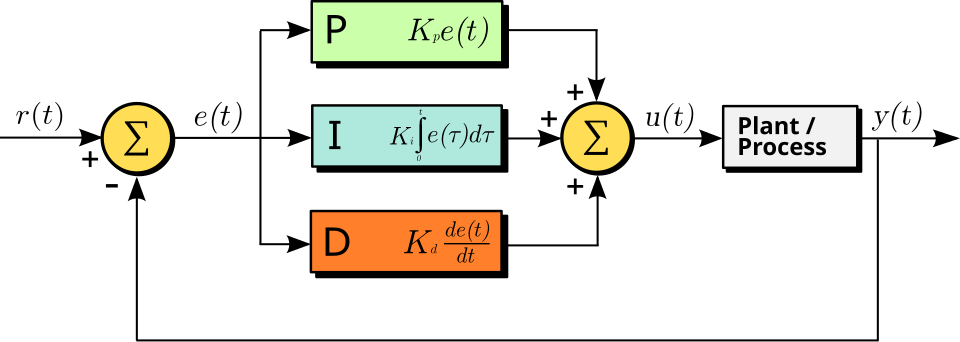
\includegraphics[width=1\columnwidth]{fig/PID_en.svg.png}
%	\caption{A block diagram of a PID controller in a feedback loop. r(t) is the desired process variable (PV) or setpoint (SP), and y(t) is the measured PV. (Wikipedia)
%		\label{fig:PID_Controller}
%	}
%\end{figure}
%
The time course of the overall control function $u(t)$ of the general \gls{PID} controller in function of the error variable $e(t)$ in Fig.~\ref{fig:PID_Controller} is
described by
\begin{equation}
	u(t)= K_p\biggl( e(t)
	+ \frac{1}{T_i} \int_0^t e(\tau) d\tau
	+ T_d \frac{de(t)}{dt}\biggr)
	\label{eq:PID}
\end{equation}
where $T_i=\frac{K_p}{K_i}$ is the time integration constant, $T_d=\frac{K_d}{K_p}$
is the derivative time constant (notice the independent time constants).
That is, in the world of a neuron, the "theory of everything" is
\begin{equation}
	V_M^{OUT}(t)= K_p\biggl( \underbrace{\overbrace{V_M^{IN}(t)}^{proportional}}_{clamping,\ synaptic}
	+ \overbrace{\underbrace{\frac{1}{T_i} \int_0^t V_{M}^{IN}(\tau) d\tau}_{membrane's\ wall}}^{integral\ (parallel\ RC)}
	+ \overbrace{\underbrace{T_d \frac{dV_M^{IN}(t)}{dt}}}^{derivative\ (serial\ RC)}_{AIS,\ synaptic}\,\biggr)
	\label{eq:PID_Neuron}
\end{equation}
The first term represents the constant effect of the external world (including synaptic inputs, clamping, and excitatory effects on brain tissue).
The second term represents the time-averaged contribution, such as 
charging up the membrane, including clamping current. The voltage is mainly due to current through ion channels in the membrane's wall; it represents a parallel $RC$ circuit. The third term represents the sum of the gradients due to all effects (the external world, the internal processes, and the outflow through the \gls{AIS}) and constitutes a serial $RC$ circuit.
The underbraces of the equation identify which components of the neuron
contribute the terms of the \gls{PID} equation.
The presence of some terms depends on the neuron's actual stage; furthermore, the $R$ values in the parallel and serial $RC$ circuit differ
(resulting in different time constants). 



One can reformulate the \gls{HH}'s famous Eq.~(1) in~\cite{HodgkinHuxley:1952} to the form of the \gls{PID} equation
\begin{equation}
	\underbrace{I \times R_{AIS}}_{V_M^{OUT}} = 
	\overbrace{\underbrace{I_i\times  R_{AIS} }_{ionic}}^{proportional}
	+\overbrace{
		\frac{1}{\underbrace{C_M\times R_{AIS}}_{T_i}} \int_0^t \xcancel{(I_{bio}-I_{clamp})(\tau)} d\tau
	}^{integral,\ clamping\ cancels\ this}
	+\overbrace{\underbrace{C_M\times R_{M}}_{T_d}\frac{dV_M}{dt}}^{derivative,\ capacitive}
	\label{eq:HH_PID}
\end{equation}
The proportional term comprises the ionic (and external) currents.
At the time when Eq.~(\ref{eq:HH_PID}) was set up, \gls{AIS} was not yet known,
so \gls{HH} assumed that in the proportional term, the resistance is identical to the membrane's resistance implemented by the ion channels in the wall (leading to the ideas of "leakage current" and "resting potential", misleading physiological research.)
The experimental conditions canceled the integral term entirely: the negative feedback from clamping precisely counterbalances the neuron's internally generated current, so the current integrates to zero.
(BTW: the "integrate and fire" type models artificially revive the forgotten
integral term.)
The derivative term assumes that all currents are constants,
so the voltage changes only due to the capacitive current.
It entirely forgets that gradients are needed to operate an
electrical system (leading to the ideas of constant-voltage batteries
and magically operated resistors in the equivalent circuits). 
Although it was known from the beginning that the \gls{AP}s comprise relatively steep rising and falling edges, it was forgotten that a non-constant current contributes a gradient to the derivative term.
\gls{HH}'s formalism describes only the 'present' (as can be expected
when freezing the state), has no predictive power, nor can it give an account of neuronal memories.


\gls{HH} considered only the proportional term, plus in the derivative term, the voltage gradient due to the condenser (but not the capacitive current itself, directly leading to the wrong ad-hoc hypothesis of the presence of $K^+$ for explaining hyperpolarization). Given that clamping obscures the presence of
gradient-like changes in the system, they missed that \textit{the input currents also produce a voltage gradient and that the output current through the \gls{AIS} also produces a gradient}. Furthermore, the equation shows that external currents (e.g., the rising and falling edges of step functions) also cause significant changes in the output voltage.
Similarly, a "foreign" invasion (changing mechanically the positions of charges by pressure, ultrasound, magnetic pulse, changing the concentration in one of the segments, and so on) generates a change in the position of charges on the neuronal membrane. This way, it generates a voltage gradient (along with pressure and other gradients), which may trigger neuronal spikes.
As discussed in section~\ref{sec:AP-PhysicalProcess},
subthreshold excitations provide direct experimental evidence that the description of the resting state includes both serial and parallel contributions.



From a control theoretical point of view, the condenser geometry and the ion concentrations set
the 'always the same' value (the setpoint; see also Figure~\ref{fig:NernstPlanckThermalWidth}) and the currents serve to keep or restore
that value.
After introducing a finite-width membrane into an electrolyte,
a potential difference between the two membrane surfaces is created; see Eq.~(\ref{eq:UGapTotal400}).
When adjusting the membrane's potential, we must consider its ground and excited states separately,
given that the perturbations in these two cases are vastly different. Nature employs various mechanisms to maintain the ground state and recover it after generating a spike. Although nature's tools are remarkably similar (channels and pumps; here, for discussing 'downhill' channels, we must consider the charge-up of different components), the significant difference in current intensity warrants a separate discussion.


When comparing Eq.~(\ref{eq:RC_Circuit_Output}) describing the operation of a simple serial $RC$ oscillator taken from the theory of electricity,  Eq.~(\ref{eq:HH_PID}) describing \gls{HH}'s differential equation
(having \gls{PID} in mind),  and the complete Eq.~(\ref{eq:PID}) describing \gls{PID} in general, one can see that they describe the 
same process in different (experimental and mathematical) approximations.
As experience shows, Eq.~(\ref{eq:RC_Circuit_Output}) describing 
the 'net electric' model provides a sufficiently accurate description
of the \gls{AP}, proving that the dominating effect comes from the derivative term and that the thermodynamic term is linearly proportional to the
electrical one. Furthermore, as we emphasized by discussing the 
physical processes and the mathematical terms, to some measure, 
the "parallel $RC$ circuit" is also present in the process, although
its current amplitude is by two orders of magnitude 
lower than that of the "serial $RC$ circuit". Furthermore, the time constants of the two circuits are also largely different, making the effect of the parallel circuit unnoticeable. 
The slow current also plays a role here: the ion currents are 'local'. 
Given that the channels in the membrane's wall are always open, the current on its way towards the \gls{AIS} may flow out
through a nearby ion channel, so only a fragment of the 'resting current' reaches the \gls{AIS}.
Eq.~(\ref{eq:PID})
provides a high-accuracy description of the process, but for most 
practical applications using Eq.~(\ref{eq:RC_Circuit_Output})
provides sufficiently good results, while Eq.~(\ref{eq:HH_PID}) is based
on an incorrect 'physical model' and requires a series of incorrect ad-hoc hypotheses to describe observations.
Note that the forces have both electrical and thermodynamic components, but they are proportional to each other. That is, although the absolute values of the coefficients in the equations are not accurate, their effects are.
Surely, the description of the processes
is complicated, but appropriate approximations give sufficiently
precise and computationally reasonable results.



\subsubsection{Robustness of the control circle}

An exciting thought experiment is discussed in~\cite{OriginMembranePotential:2017}. "First, we consider a hypothetical membrane that is permeable only to $Na^+$ ions. Suppose that $[Na^+]_o$, the outside or extracellular sodium concentration, is $145\ mM$, and $[Na^+]_i$ is 12 mM. Moreover, suppose that initially, there is no membrane potential. The diffusion gradient for $Na^+$ favors $Na^+$ entry into the cell, and the initial $Na^+$ influx carries a charge that builds up on the inside of the cell. This produces a potential (recall that separation of charge produces a potential) across the membrane that impedes further $Na^+$ ion movement because the positive charges repel the positively charged $Na^+$ ion."

The paper correctly explains that in the case of $Na^+$ only, the potential is set up
to $66.6\ mV$. (We quietly add that plus a layer of the corresponding $Cl^-$ ions on the other segment, in a similar concentration ratio, builds up; so also, the attraction between positive and negative charges contributes to the effect.) 
In the absence of our argumentation, it cannot explain \textit{why} 
that potential builds up; only why that concentration ratio
establishes: the Nernst law alone does not explain the effect. Furthermore, the statement is valid only for
a well-defined semipermeable membrane.
We can add that the same concentrations develop if initially identical concentrations
are present on both sides. 
The finite width of the membrane creates an electrical potential, a consequence of charge separation, as stated. 
If there are no ions initially inside, then no charge separation occurs, and therefore, no ion transport begins due to the membrane's electrical potential. However, the thermal driving force exists, and the started ion transport quickly builds the electrical layer, which effectively helps to establish the resting potential. 

This robustness also explains why, during replication (cell division), cells also inherit their operating ability and resting potential; the existing membrane cell continues to grow in the same way. Its voltage does not depend on its size, so it remains constant, and the voltage defined in this way adjusts the concentrations accordingly. Moreover, it explains why, during evolution, cells first formed: a couple of lipids came together to form an imperfect membrane with holes, establishing cellular electricity. As Fig.~\ref{fig:RestingPotential3} depicts, the concentrations may adapt to the living conditions (whether living in seawater), but the general operating principles remain the same. The seawater environment 
enables the use of thinner membranes and lower membrane voltages; however, the same electrical field is used in all cases.

Given that neurons share the external (global) concentrations (defined by the vast amount of ions in the bulk), they provide a firmly fixed offset value to the always-the-same electrical potential. This way, the operations of the individual neurons do not interfere. Furthermore, the internal (local) concentrations can adjust themselves even following a very rough charge perturbation
while issuing an \gls{AP}; moreover, when the living organism is growing.

\subsection{Goldman-Hodgkin-Katz potential\label{sec:Goldman-Hodgkin-Katz}}


It has already been stated, based on experimental evidence, that "the membrane permeability to the ions has nothing to do with the potential generation and the ions' adsorption on the membrane surface generates the membrane potential"; for a review, see~\cite{MembranePotentialPermeability:2024}.
The idea itself is nonsense: in a balanced state, no ion transport happens, so even without permeability, the balanced state persists;  the resting potential has nothing to do with either ions' mobility or permeability or with ion absorption~\cite{Hodgkin-HuxleyAdsorption:2021}.
Furthermore, there is no idea in \gls{GHK} about whether the 'setpoint' (why that specific concentration or potential difference) is present and why the same potential is reset after rough perturbations such as issuing an \gls{AP} or replicating a cell.
The causality is reversed: the potential is a static concept and is set electrically, and
the two gradients form the experienced concentrations from the available solvent molecules.
For the time course of gradient formation, mobility and permeability play a role, but not in determining concentrations or the resting potential.

In our clear physical picture, the thermodynamic forces on one side
and on the other side of the membrane are summed. They counterbalance each other; furthermore, jointly the effect of the neuronal condenser, see  Fig.~\ref{fig:RestingPotential3}.
As we emphasized, the concentration gradients are ion-specific.
Furthermore, as discussed in connection with Eq.(\ref{eq:Nernst1}), the Nernst equation comprises a per-ion indefinite constant (a potential difference).
To calculate a linear combination of terms comprising an arbitrary constant is nonsense,
and so is adding absolute concentrations on the different sides of the membrane, or changing the base of the logarithm used in a calculation to match
the experimental value. It is not more than number magic. The potential is described by coupled equations as discussed in connection with Eq.~(\ref{eq:coupling}).

The $Ca^{2+}$ ions do not fit into the \gls{GHK} picture. 
One of the reasons why \gls{GHK} cannot be good is that $[Ca^{2+}]$
is omitted. Biologically, it is hard to believe that $Ca^{2+}$ does not participate in the game of life (especially since biology sees the need for $Ca^{2+}$ pumps). Physically, a single concentration on one side of the membrane cannot maintain balance; as the different ion-exchange processes shown in Table~\ref{Tab:SummaryTable} and Fig.~\ref{fig:RestingPotential3} demonstrate.
When adding a new ion to the solution, the sum concentration
increases, and so the electrical force increases, forcing the previous 
elements to find new concentrations on both sides.
The appearance of a new chemical element indirectly changes the concentrations of the others (a good example is the role of the negligible amount of $Ca^{2+}$).


\physicspanel{phys:EquivalentField_GHK}{The effect of Nernst-Plack law on the GHK equation}
{
\paragraph{Warning}

The potential derived in \hyperlink{phys:Nernst-Planck}
{\textbf{Physics panel~\ref{phys:Nernst-Planck}}}
 inherently comprises an additive term (a potential difference), so they must not be compared directly if they use a different reference $C_{k}^{int}$
(furthermore, it is nonsense to combine  quantities from the intracellular and extracellular sides additively,
whether concentrations, mobilities, or Nernst voltages, as it happens in the \gls{GHK} equation (see section~\ref{sec:Goldman-Hodgkin-Katz}).

The derivatives are spatial derivatives; the temporal derivatives (needed for describing the time course) of the concentration(s) and voltage are derived in~\cite{VeghNonOrdinaryLawsForLife:2025}. 
In 'ordinary' physics, where the charge and mass are independent,
changing one side changes the other in the opposite direction.
In 'non-ordinary' physics~\cite{VeghNon-ordinaryLaws:2025}, valid for electrolytes, the two differentials must change in the same direction,
given that ions' charge and mass cannot be separated 
(BTW: this is why Eq.~(\ref{eq:Nernst1}) results in a negative potential difference).
(The derivation in 'ordinary physics', such as ~\cite{KochBiophysics:1999},
Eq.(11.30), is wrong, at least because of two reasons: the same speed is assumed for mass and charge transport; furthermore, the used partial derivatives are not independent; the details are discussed throughout the paper.)
}

\ifx\magyar\undefined
\numericspanel{phys:ForceFromElasticMembrane}{The elastic force}
{
For this calculation
we can use the identity that
\\
\SI{1}{\volt\per\meter}
== \SI{1}{\newton\per\coulomb} == \SI{1}{\meter\kg\per\sec^2 \per\coulomb}
\\
A $100~mV$ damped oscillation of $1 kHz$ (1 msec period) has the form ($A$ is the amplitude of the motion of an ion
\\
$A(t)=A\times e^{-\zeta*t}\times cos(\omega\times t)$
\\ Here we do not consider the discharge process for the moment.
\\Dividing with the mass of ion and multiplying with its charge, 

We assume that moving $10^7$ charges with frequency $\omega$ and amplitude $A$ generate the voltage, and calculate the
time derivative (for a moment we omit the discharge tag)

\[
\frac{10^{-1}}{10^7} \bigg[\frac{V}{m}\bigg] \bigg[\frac{1}{s}\bigg]
= A\times \frac{3.86\times 10^{-26}}{1.6\times 10^{-19}} \times \omega \bigg[\frac{1}{s}\bigg] \times sin (\omega\times t) \bigg[\frac{m}{s^2}\bigg]
\]

that is
\[
1\ [V] 
= A[m] \times 2.4 \times \omega \times sin (\omega\times t) \bigg[\frac{m}{s^2}\bigg]
\]

and the second derivative
\[
1\ [V]
= A[m] \times 2.4 \times \times \omega^2 \times cos (\omega\times t) \bigg[\frac{m}{s^2}\bigg] \bigg[\frac{1}{s}\bigg]
\]


with frequency $\omega$
\[
1[V] 
= \frac{A}{1.6\times 10^{-11}} \times \omega^2 \times cos (\omega\times t) \bigg[\frac{kg\times m}{s^2}\bigg] \]

Since $\omega=10^{3}$,

\[
1 [V] 
= \frac{A\,[m]}{1.6\times 10^{-5}} \times cos (\omega\times t) \bigg[\frac{kg\times m}{s^2}\bigg] 
\]

That is, the amplitude of the motion of an ion is about $0.2\ \mu m$. Using the second derivative, we can estimate the (maximal) force: 
\[
	F [N] = 3.82 \times 10^{-26} [kg]\times 1.6 \times 10^{-5} \times (10^3)^2 \bigg[\frac{m}{s^2}\bigg]
\]
The maximum force from the elastic wave is
\[
F = 6\times 10^{-25} [N] 
\]

Compare the value to \textbf{\hyperlink{phys:CellForceinField}{Physics Panel~\ref{phys:CellForceinField}}}
}

\else



\numericspanel{phys:ForceFromElasticMembrane}{A rugalmas erő}
{

Amint a  
\textbf{\hyperlink{phys:CellForceinField}{Numerics panel~\ref{phys:CellForceinField}}} bemutatta, a rush-in utáni 
pillanatban egy ion $F_{max} = 1.6*10^{-12}\ [N]$ erőt fejt ki a membránra.
A membrán ugyanekkora kényszererőt fejt ki az ionra. 
A membrán mozgását leíró egyenlet által meghatározva, az ionra ható rugalmas erőt a
\[
F(t) = F_{max}\times e^{-\zeta*t}\times cos(\omega\times t)
\]
\noindent 
egyenlet adja meg. A \textbf{\hyperlink{phys:RushinSpeed}{Numerics panel~\ref{phys:RushinSpeed}}} szerint a rush-in után az \gls{AIS}-en
legfeljebb
%
\begin{equation}
	F_{Na^+}= 2*10^3  [N/C] \times 1.602* 10^{-19} [C] = 3.2*10^{-16}\ [N] \label{eq:ElecticForce}
\end{equation}
%
\noindent
elektromos erő mozgatja az ionokat. A rush-in által generált gradiens és
erő kb. ugyanilyen nagyságú, hasonlóan a termodinamikai gradiens is.
Eszerint a maximális rugalmas mozgató erő több mint két nagyságrenddel nagyobb mint a maximális elektromos erő, így a csillapított rugalmas rezgés szinte tökéletesen leírja az \gls{AP}-t. A rugalmas erő oszcillál, ezért annak domináns hatása nem állandó.

%Ehhez a számításhoz felhasználjuk a
%\\
%\SI{1}{\volt\per\meter}
%== \SI{1}{\newton\per\coulomb} == \SI{1}{\meter\kg\per\sec^2 \per\coulomb}
%\\
%azonosságát. Egyszerűsített fizikai képünkben $10^7$ ion együttes rezgőmozgása
%generálja a mérhető, $\omega$ frekvenciájú $V_{max}$  elektromos hullámot, amelyben az ionok $A$ amplitúdóval mozognak. A rezgőmozgásból eredő feszültséghullámot a
%
%\[
%V(t) = V_{max}\times e^{-\zeta*t}\times cos(\omega\times t)
%\]
%\noindent
%formula írja le. A $10^7$ ion $A$ távolságban 
%\[
%E \bigg[\frac{V}{m}\biggr]=\frac{e_{el}}{4\times \pi\times \epsilon_\circ \times A^2}
%= 9\times 10^9 \big[\frac{N\,m^2}{C^2}\big] \times \frac{1.6\times 10^{-19} [C]}{A^2 [{m^2}]}
%\]
%\[
%E \bigg[\frac{V}{m}\biggr] = \frac{14.4\times 10^{-10}}{A^2}\bigg[\frac{N}{C}\biggr] = \frac{14.4\times 10^{-10}}{A^2}\bigg[\frac{V}{m}\biggr]
%\]
%\noindent
%nagyságú teret gerjesztenek. Az $A$ távolságban
%\[
%10^{-1} [V]= E\times A [V] = \frac{14.4\times 10^{-10}}{A} 
%\]
%\noindent 
%feszültséget gerjeszt, amiből 
%\[
%A= 14.4 [nm]
%\]
%
%A fenti formulából, kétszeres deriválás után a gyorsulás 
%\[
%	a_{Na^+} = \frac{d^2 z}{dt^2} = A \omega^2 cos(\omega\times t)
%	=  14.4 \times 10^{-9}\times 10^6 = 14.4 \times 10^{-3} \bigg[\frac{m}{s^2}\biggr]
%\]
%
%From Newton's 2nd law,
%\[
%F_{elastic} = m_{Na^+}\times a_{Na^+} = 10^{-26} \times 14.4 \times 10^{-3} \bigg[\frac{kg\,m}{s^2}\biggr]
%\]
%%\[
%%%	F_{elastic} = m_{Na^+}\times a_{Na^+}
%%\]
%
%% 
%
%% (az egyszerűség kedvéért az emponenciális tag nélkül) 
%%A $100~mV$ damped oscillation of $1 kHz$ (1 msec period) has the form ($A$ is the amplitude of the motion of an ion
%%\\
%%\\ Here we do not consider the discharge process for the moment.
%%\\Dividing with the mass of ion and multiplying with its charge, 
%%
%%We assume that moving $10^7$ charges with frequency $\omega$ and amplitude $A$ generate the voltage, and calculate the
%%time derivative (for a moment we omit the discharge tag)
%%
%%\[
%%\frac{10^{-1}}{10^7} \bigg[\frac{V}{m}\bigg] \bigg[\frac{1}{s}\bigg]
%%= A\times \frac{3.86\times 10^{-26}}{1.6\times 10^{-19}} \times \omega \bigg[\frac{1}{s}\bigg] \times sin (\omega\times t) \bigg[\frac{m}{s^2}\bigg]
%%\]
%%
%%that is
%%\[
%%1\ [V] 
%%= A[m] \times 2.4 \times \omega \times sin (\omega\times t) \bigg[\frac{m}{s^2}\bigg]
%%\]
%%
%%and the second derivative
%%\[
%%1\ [V]
%%= A[m] \times 2.4 \times \times \omega^2 \times cos (\omega\times t) \bigg[\frac{m}{s^2}\bigg] \bigg[\frac{1}{s}\bigg]
%%\]
%%
%%
%%with frequency $\omega$
%%\[
%%1[V] 
%%= \frac{A}{1.6\times 10^{-11}} \times \omega^2 \times cos (\omega\times t) \bigg[\frac{kg\times m}{s^2}\bigg] \]
%%
%%Since $\omega=10^{3}$,
%%
%%\[
%%1 [V] 
%%= \frac{A\,[m]}{1.6\times 10^{-5}} \times cos (\omega\times t) \bigg[\frac{kg\times m}{s^2}\bigg] 
%%\]
%%
%%That is, the amplitude of the motion of an ion is about $0.2\ \mu m$. Using the second derivative, we can estimate the (maximal) force: 
%%\[
%%	F [N] = 3.82 \times 10^{-26} [kg]\times 1.6 \times 10^{-5} \times (10^3)^2 \bigg[\frac{m}{s^2}\bigg]
%%\]
%%The maximum force from the elastic wave is
%%\[
%%F = 6\times 10^{-25} [N] 
%%\]
%%
%%Compare the value to \textbf{\hyperlink{phys:CellForceinField}{Physics Panel~\ref{phys:CellForceinField}}}
}
\fi
\input{src/MembraneActionPotential}

